\documentclass[a4paper]{article}
% \documentclass{book}
\usepackage[utf8]{inputenc}
\usepackage[T2A]{fontenc}
\usepackage[english, russian]{babel}
\usepackage[left=25mm, top=20mm, right=25mm, bottom=30mm, nohead, nofoot]{geometry}
\usepackage{amsmath, amsfonts, amssymb} % математический пакет
\usepackage {fancybox, fancyhdr}
\pagestyle{fancy}
\fancyhf{}
\fancyhead[R]{Винер Даниил. БЭАД232}
\fancyfoot [R] {\thepage}
\fancyhead[L]{Дискретная математика. Коллоквиум-1}
\setcounter {page}{1}
\headsep=10mm
\usepackage{xcolor}
\usepackage{blindtext}
\usepackage {hyperref}
\hypersetup{colorlinks=true, allcolors= [RGB]{010 090 200}} % цвет ссылок
\usepackage {setspace}
\usepackage[pdftex]{graphicx}
\usepackage{ dsfont }
\usepackage{array}
\setcounter{MaxMatrixCols}{20}
\usepackage{enumerate}
\usepackage{listings}
\usepackage{color}
\definecolor{dkgreen}{rgb}{0,0.6,0}
\definecolor{gray}{rgb}{0.5,0.5,0.5}
\definecolor{mauve}{rgb}{0.58,0,0.82}
\lstset{frame=tb,
  language=Python,
  aboveskip=3mm,
  belowskip=3mm,
  showstringspaces=false,
  columns=flexible,
  basicstyle={\small\ttfamily},
  numbers=none,
  numberstyle=\tiny\color{gray},
  keywordstyle=\color{blue},
  commentstyle=\color{dkgreen},
  stringstyle=\color{mauve},
  breaklines=true,
  breakatwhitespace=true,
  tabsize=3
}
\usepackage{tabularx}
\usepackage{multirow}
\usepackage{ upgreek }
\usepackage{tikz}
\newcommand{\qed}{\hfill$\square$}

\makeatletter
\newcommand\binomialCoefficient[2]{%
    % Store values 
    \c@pgf@counta=#1% n
    \c@pgf@countb=#2% k
    %
    % Take advantage of symmetry if k > n - k
    \c@pgf@countc=\c@pgf@counta%
    \advance\c@pgf@countc by-\c@pgf@countb%
    \ifnum\c@pgf@countb>\c@pgf@countc%
        \c@pgf@countb=\c@pgf@countc%
    \fi%
    %
    % Recursively compute the coefficients
    \c@pgf@countc=1% will hold the result
    \c@pgf@countd=0% counter
    \pgfmathloop% c -> c*(n-i)/(i+1) for i=0,...,k-1
        \ifnum\c@pgf@countd<\c@pgf@countb%
        \multiply\c@pgf@countc by\c@pgf@counta%
        \advance\c@pgf@counta by-1%
        \advance\c@pgf@countd by1%
        \divide\c@pgf@countc by\c@pgf@countd%
    \repeatpgfmathloop%
    \the\c@pgf@countc%
}
\makeatother

\begin{document}

\tableofcontents

\newpage
\section{Определения и формулировки}
\subsection{Таблица истинности логических связок}

\begin{tabular}{|c|c|c|c|c|c|}
\hline
$A$ & $B$ & $A\wedge B$ & $A\vee B$ & $A\rightarrow B$ & $A\equiv B$ \\
\hline
0 & 0 & 0 & 0 & 1 & 1 \\
\hline
0 & 1 & 0 & 1 & 1 & 0 \\
\hline
1 & 0 & 0 & 1 & 0 & 0 \\
\hline
1 & 1 & 1 & 1 & 1 & 1 \\
\hline
\end{tabular}
\subsection{Равносильные высказывания. Тавтологии}
Если два разных составных высказывания означают по сути одно и то же, то есть принимают одинаковое логическое значение при одинаковых значениях входящих в них элементарных высказываний. В этом случае мы говорим, что высказывания \textit{равносильны}\\[2mm]
\indentВысказывание, которое истинно при любых значениях входящих в него элементарных высказываний называется \textit{\textbf{тавтологией}}. Тавтологии не обязательно имеют вид логических тождеств. Например, $A\rightarrow A$ — тавтология
\subsection{Коммутативность и ассоциативность конъюнкции и дизъюнкции}
Коммутативность: $A\wedge B\equiv B\wedge A,\ A\vee B\equiv B\vee A$\\[2mm]
Ассоциативность: $(A\wedge B)\wedge C\equiv A\wedge (B\wedge C),\ (A\vee B)\vee C\equiv A\vee (B\vee C)$\\[2mm]
\indentСправедливость этих тождеств ясна из  определения конъюнкции и дизъюнкции. Первая истинна, когда все члены истинны (необязательно членов два), вторая — когда хотя бы один истинен
\subsection{Тавтологии упрощения для $\wedge, \vee, \rightarrow$}
Пусть $X$ - константа, тогда имеем \textit{тавталогии упрощения}:\\[2mm]
$X\wedge 0\equiv 0,\ X\wedge 1\equiv X\\[2mm]
X\vee 0\equiv X,\ X\vee 1\equiv 1\\[2mm]
X\rightarrow1\equiv1,\ X\rightarrow0\equiv\neg X\\[2mm]
0\rightarrow X\equiv1,\ 1\rightarrow X\equiv X\\[2mm]$
Их справедливость очевидна из таблиц истинности связок\\[2mm]
Некоторые теоремы о тавтологиях доказываются здесь - \ref{sec:2.2}
\subsection{Тавтология для правила modus ponens. Закон контрапозиции}
\indent\textbf{Правило modus ponens} можно записать в виде такой тавтологии: $A\wedge (A\rightarrow B)\rightarrow B$\\[2mm]
\indentЭто правило описывает стандартный шаг математического рассуждения, что из истинности высказывания $A$ и составного высказывания \guillemotleftесли $A$, то $B$\guillemotright, мы говорим, что истинно $B$\\[2mm]
\indent\textbf{Закон контрапозиции:} $A\rightarrow B\equiv\neg B\rightarrow\neg A$\\[2mm]
Некоторые теоремы о тавтологиях доказываются здесь - \ref{sec:2.2}
\subsection{Дистрибутивность конъюкции и дизъюнкции}
\textbf{Первый:} $A\wedge(B\vee C)\equiv(A\wedge B)\vee(A\wedge C)$\\[2mm]
\textbf{Второй:} $A\vee(B\wedge C)\equiv(A\vee B)\wedge(A\vee C)$\\[2mm]
Доказательство - \ref{sec:2.1}
\subsection{Равные множества. Подмножество. Пустое множество}
% \textbf{\textit{Множество}} — это совокупность каких-то элементов. Природа элементов и взаимоотношения между ними не важны. Существенно лишь, какие элементы входят в множество, а какие — нет, то есть множество полностью определяется своими элементами\\[2mm]
\indent\centerline{$A=B \stackrel{\text{def}}{\Leftrightarrow}\forall x(x\in A\equiv x\in B)$}\\[2mm]
\indentМножества $A$ и $B$ называются \textbf{\textit{равными}}, если каждый элемент множества $A$ является элементом множества $B$, а каждый элемент множества $B$ является элементом множества $A$\\[2mm]
\centerline{$A\subseteq B \stackrel{\text{def}}{\Leftrightarrow}\forall x(x\in A\rightarrow x\in B)$}\\[2mm]
\indentМножество $A$ является \textbf{\textit{подмножеством}} множества $B$, если каждый элемент множества $A$ принадлежит множеству $B$ (обозначение $A\subseteq B$)\\[2mm]
\indent\textbf{Пустое множество} (обозначение $\varnothing$) не содержит ни одного элемента.
Другими словами, высказывание $x\in\varnothing$ ложно для любого $x$
\subsection{Операции над множествами: объединение, пересечение, разность, симметрическая разность}
Имеем два множества: $A$ и $B$. С ними можно выполнять следующие опреации:\\[2mm]
\indent \textbf{Объединение множеств.} $A\cup B$. Это множество, состоящее из тех элементов, которые принадлежат хотя бы одному из множеств $A$ и $B$. Формально это определение выглядит так:\\[2mm] \centerline{$(x\in A\cup B)\equiv(x\in A)\vee(x\in B)$}\\[2mm]
\indent \textbf{Пересечение множеств.} $A\cap B$. Это множество, состоящее из тех элементов, которые принадлежат обоим множествам $A$ и $B$. Формально:\\[2mm]
\centerline{$(x\in A\cap B)\equiv(x\in A)\wedge(x\in B)$}\\[2mm]
\indent \textbf{Разность множеств.} $A\setminus B$. Это множество, состоящее из тех элементов, которые принадлежат множеству $A$, но не принадлежат множеству $B$. В формальной записи это определение выглядит так:\\[2mm]
\centerline{$(x\in A\setminus B)=(x\in A)\wedge \neg(x\in B)$}\\[2mm]
\indent \textbf{Симметрическая разность множеств.} $A\triangle B$. Это множество, состоящее из тех элементов, которые принадлежат ровно одному из множеств: либо $A$, либо $B$. Формально:\\[2mm]
\centerline{$(x\in A\triangle B)=((x\in A)\wedge\neg(x\in B))\vee(\neg(x\in A)\wedge(x\in B))$}
\subsection{Неформальное определение конечного множества и подсчёта}
\indent\textbf{Конечное множество} — это такое множество, в котором конечное количество элементов, то есть оно \textit{конечно}, если его элементы можно \textit{пересчитать}\\[2mm]
\indent Неформально \textit{подсчёт} осуществляется так: «вот первый элемент, вот второй, вот третий, ...». Если такой подсчёт заканчивается, то последнее названное число и будет количеством элементов в множестве, т.е. множество конечно\\[2mm]
\indent Более строгое описание подсчёта такое: это такая последовательность элементов множества $(a_1, a_2, \ldots, a_n)$ в которой все элементы различны, принадлежат множеству и каждый элемент множества входит в последовательность (причём ровно один раз)
\subsection{Правило суммы. Декартово произведение множеств. Правило произведения}
\textbf{Правило суммы.} Для конечных непересекающихся множеств $A,\ B$ ($A\cap B=\varnothing$) выполняется равенство $|A\cup B|=|A|+|B|$\\[2mm]
\indent \textbf{Декартово произведение множеств.} ($A\times B$). Это множество, состоящее в точности из всех таких упорядоченных пар $(a,\ b)$, то есть последовательностей длины $2$, в которых $a\in A,\ b\in B$. Если множества конечны, то декартово произведение можно нарисовать в виде прямоугольника: столбцы — элементы $A$, строки — элементы $B$, на пересечении столбца $a$ и строки $b$ расположена пара $(a,\ b)\in A\times B$\\[2mm]
\indent \textbf{Правило произведения.} Для конечных множеств $A,\ B$ выполняется равенство $|A\times B|=|A|\cdot|B|$
\subsection{Тавтологии: транзитивность импликации, доказательство от противного}
\textbf{Транзитивность импликации:} $((A\rightarrow B)\wedge(B\rightarrow C))\rightarrow(A\rightarrow C)$\\[2mm]
\indent \textit{Доказать от противного} можно эту же тавтологию. Предположим, что высказывание ложно при каких-то значениях элементарных высказываний\\[2mm]
\indentИз таблицы истинности импликации видим, что тогда заключение $A\rightarrow C$ внешней импликации ложно, а посылка $(A\rightarrow B)\wedge(B\rightarrow C)$ истинна\\[2mm]
\indentИз ложности $A\rightarrow C$ заключаем, что $A=1$, $C=0$. Истинность конъюнкции означает, что истинны оба члена конъюнкции, в частности $B\rightarrow C=B\rightarrow0=1$. Это возможно лишь при $B=0$. Но тогда $A\rightarrow B=1\rightarrow0=0$, а мы уже установили, что $A\rightarrow B=1$. Пришли к противоречию. \qed\\[2mm]
\subsection{Законы де Моргана. Аналоги законов де Моргана для кванторов}
Тавтологии $\neg(A\wedge B)\equiv\neg A\vee\neg B,\ \neg(A\vee B)\equiv\neg A\wedge\neg B$ называются \textit{законами де Моргана}\\[2mm]
\indent \textbf{Аналоги законов для кванторов:} $\neg\forall xA(x)\equiv\exists x\neg A(x),\ \neg\exists xA(x)\equiv\forall x\neg A(x)$
% Законы де Моргана доказываются здесь - \ref{sec:2.3}
\subsection{Ограниченные кванторные высказывания и их запись через неограниченные кванторные высказывания}
В ограниченном кванторном высказывании $x$ пробегает не все возможные значения, а лишь множество, ограниченное некотррым условием. Формальная запись такова:\\[2mm]
\centerline{$\forall x\in A\ B(x)$ и $\exists x\in A\ B(x)$}\\[2mm]
\indent В неограниченных кванторных высказываниях это выглядит так: \\[2mm]
\centerline{$\forall x(x\in A\rightarrow B(x))$ и $\exists x(x\in A\wedge B(x))$}
\subsection{Принцип математической индукции}
\label{sec:1.14}\textbf{Принцип математической индукции.} Пусть для последовательности утверждений $A_0, A_1,\ldots, A_n, \ldots$, занумерованных натуральными числами, верны утверждения\\[2mm]
\indent \textbf{База индукции:} $A_0$ истинно
\indent \textbf{Шаг индукции:} $A_N\rightarrow A_{n+1}$ истинно для любого $n$. Посылку импликации $A_n$ называют индуктивным предположением. Тогда $A_n$ истинно $\forall n$\\[2mm]
\indentПоложим, что $n$ принимает только натуральные значения и запишем это в виде формулы (вместо $A_n$ пишем $A(n)$:\\[2mm]
\centerline{$(A(0)\wedge\forall n(A(n)\rightarrow A(n+1)))\rightarrow\forall nA(n)$}\\[2mm]
Доказательство - \ref{sec:2.4}
\subsection{Принцип полной математической индукции}
\label{sec:1.15}Пусть для последовательности утверждений $A_0, A_1, \ldots, A_n, \ldots$, занумерованных натуральными числами, истинно утверждение: \guillemotleft для любого $n$ из истинности $A_i$ при всех $i<n$ следует истинность $A_n$\guillemotright. Тогда $A_n$ истинно $\forall n$\\[2mm]
\indent В виде формулы это можно записать так: \\[2mm]
\centerline{$\forall n((\forall k<n\ A(k))\rightarrow A(n))\rightarrow\forall nA(n)$}
\subsection{Упорядоченная пара по Куратовскому}
\label{sec:1.16}Для упорядоченных пар выполняется свойство: $(x_1, y_1)=(x_2,y_2)\Leftrightarrow x_1=x_2,\ y_1=y_2$\\[2mm]
Упорядоченной парой по Куратовскому $(x,y)$ будем называть
множество $\{\{x\},\{x,y\}\}$\\[2mm]
Доказательство - \ref{sec:2.5}
\subsection{Бинарное отношение на множествах $A$ и $B$. Бинарное отношение на множестве $A$}
Бинарное отношение $R$ на множествах $A$ и $B$ - это подмножество декартового произведения $A\times B$\\[2mm]
\indent Если $(x,y)\in R$, то говорят, что $x$ и $y$ находятся в отношении $R$ (порядок важен). Вместо $(x,y)\in R$ также пишут $xRy$\\[2mm]
\indent Бинарное отношение $R$ на множетсвах $A, A$ называют бинарным отношением на множестве $A$
\subsection{Функция. Аргументы и значения}
Функцией $f$ из множества $A$ в множество $B$ будем называть такое бинарное отношение $f\subseteq A\times B$, что для каждого $a\in A$ есть не более одной пары $(a, b)\in f$\\[2mm]
\indent Элементы множества $A$ называются \textit{аргументами} функции, а элементы множества $B$ - \textit{значениями} функции
\subsection{Область определения функции. Область значений функции. Тотальные функции}
\textbf{Область определения} Dom $f$ функции из $A$ в $B$ - это множество тех $a$, для которых существует такой $b$, что $(a, b)\in f$. Формальная запись такова:\\[2mm]
\centerline{Dom$(f)=\{x\in A\ |\ \exists y\in B: y=f(x)\}$}\\[2mm]
\indent Если Dom$(f)=A$, то функция называется \textit{\textbf{тотальной}} (=всюду определнной). Нетотальные функции называют \textit{частичными}\\[2mm]
\indent \textbf{Область значений} Range$f$ - это множество тех $b$, для котороых существует такой $a$, что $(a, b)\in f$. Формальная запись определния такова:\\[2mm]
\centerline{Range$(f)=\{y\in B\ |\ \exists x\in A: y=f(x)\}$}
\subsection{Начальный отрезок натурального ряда. Конечная последовательность элементов множества $A$. Бесконечная последовательность элементов множества $A$}
\textbf{Начальный отрезок натурального ряда} - множество вида $[n]=\{x: x<n, x\in\mathbb{N}\}$. Оно состоит из чисел $0, 1, \ldots, n-1,$ всего $n$ чисел\\[2mm]
\indent \textbf{Конечная последовательность элементов множества $A$} - это тотальная функция $[n]\rightarrow A$\\[2mm]
\indent \textbf{Бесконечная последовательность элементов множества $A$} - тотальная функция $\mathbb{N}\rightarrow A$
\subsection{Инъекция. Примеры инъекции и не инъекции}
\textbf{Инъекция} - тотальная функция $f: A\rightarrow B$, если значения функции в различных точках различны. То есть: $f-$инъекция, если $x_1\ne x_2$ влечет $f(x_1)\ne f(x_2)$\\[2mm]
\indent \textbf{Пример:} пусть $f: \mathbb{N}\rightarrow\mathbb{N}$ задается формулой $f(x)=x^2$. Эта функция, во-первых, тотальна, а во-вторых, инъективна, так как если $x_1, x_2\in \mathbb{N}$ и $x_1^2=x_2^2$, то $x_1=x_2$\\[2mm]
\indent \textbf{Контрпример:} $g: \mathbb{R}\rightarrow\mathbb{R},\ g(x)=x^2$. Она также тотальная, но не инъективна, так как $g(-1)=g(1)=1$
\subsection{Сюръекция. Примеры сюръекции и не сюръекции}
\textbf{Сюръекция} - тотальная функция $f: A\rightarrow B$, если область значений совпадает со всем множеством $B$, то есть Range$f=B$. Другими словами, $f$ сюръекция, если для всякого элемента $y\in B$ найдется такой элемент $x\in A$, что $f(x)=y$\\[2mm]
\indent \textbf{Пример:} рассмотрим функцию $g: \mathbb{R}\rightarrow\mathbb{R}_{\geqslant0}$, задаваемую формулой $g(x)=x^2$. Эта функция тотальна и сюръективна, так как для любого $y\in\mathbb{R}_{\geqslant0}$ существует $x\in\mathbb{R}$, что $x^2=y$\\[2mm]
\indent \textbf{Контрпример:} рассмотрим функцию $f: \mathbb{R}\rightarrow\mathbb{R}$, задваемую той же формулой. Эта функция тотальна, но не сюръективна, так каак не существует такого $x\in \mathbb{R}$, при котором $f(x)=-1$
\subsection{Биекция. Обратная функция}
Тотальная функция $f: A\rightarrow B$ называется \textit{биекцией}, если она одновременно является инъекцией и сюръекцией\\[2mm]
\indent Для биекции $f: A\rightarrow B$ определена \textbf{\textit{обратная функция}} $f^{-1}:$ если $f$ отображает $x$ в $y$, то обратная функция $f^{-1}$ отображает $y$ в $x$. Иными словами, $(x, y)\in f\Leftrightarrow(y, x)\in f^{-1}$\\[2mm]
% \indent \textbf{Примечание:} мы определили некоторый объект $f^{-1}$, про который мы можем сказать только то, что он является бинарным отношением на множествах $B$ и $A$. $f^{-1}$  также являеся биекцией, но это нужно доказать
\subsection{Композиция функций. Ассоциативность композиции}
Для функции $f: A\rightarrow B$ и функции $g: B\rightarrow C$ \textit{композицией} $g\circ f$ этих функций является такая функция $A\rightarrow C$, которая определена на тех $x$ из Dom$(f)$, для которых $f(x)$ принадлежит Dom$(g)$, и равна $g(f(x))$. Формальная запись выглядит так:\\[2mm]
\centerline{$(x,z)\in g\circ f\Leftrightarrow\exists y\in B: (x,y)\in f$ и $(y,z)\in g$}\\[2mm]
\indent Порядок записи функций в композиции согласован с порядком записи функций
в привычном обозначении $g(f(x))$ и порядок функций в композиции важен\\[2mm]
\indent \textbf{Ассоциативность композиции:} $(f\circ g)\circ h=f\circ (g\circ h)$\\[2mm]
\indent \textbf{Пример композиции.} Пусть $f(x)=x+1, g(x)=2x$ — функции из целых чисел в целые
числа. Тогда $(g\circ f)(x)=2x+2,\ (f\circ g)(x)=2x+1$
\subsection{Принцип Дирихле}
Принцип Дирихле можно представить на кроликах\\[2mm]
\indent Если $k>n$ и $k$ кроликов рассажены по $n$ клеткам, то хотя бы в одной клетке сидит как минимум два кролика\\[2mm]
\indent Более формально (занумеруем клетки, и пусть в клетку с номером $i$ посажено $r_i$ кроликов): Если $k>n,\ r_1,\ldots,r_n$ - натуральные числа и $r_1+\ldots+r_n=k$, то для какого-то $i$ выполняется неравенство $r_i>1$
\subsection{Конечное множество. Мощность конечного множества}
\label{sec:intro}
Множество $A$ называется \textit{конечным}, если для некоторого натурального $n$ существует биекция $f: [n]\rightarrow A$\\[2mm]
Число $n$ называется размером (=мощностью) $A$ и обозначается $|A|$
\subsection{Образ и полный прообраз}
Пусть $X\subseteq A$. Функция $f$ сопоставляет ему \textbf{\textit{образ}} $f[X]\subseteq B$ подмножества $X$. По определению $f[X]$ состоит в точности из тех элементов множества $B$, которые являеются значениями элементов из $X$. Формально это выгялдит так:\\[2mm]
\centerline{$f[X]=\{b\in B\ |\ \exists x\in X: b=f(x)\}$}\\[2mm]
\indent Заметим, что если в качестве $X$ взять само множество $A$, то легко увидеть, что $f[A]={Range}(f)$\\[2mm]
\indent Пусть $Y\subseteq B$. Полный прообраз $f^{-1}[Y]$ состоит в точности из тех элементов $A$, значения которых лежат в $Y$. Запишем формально:\\[2mm]
\centerline{$f^{-1}[Y]=\{a\in A: f(a)\in Y\}$}\\[2mm]
\indent Аналогично образу, нетрудно заметить, что $f^{-1}[B]=Dom(f)$, то есть прообраз всего множества $B$ совпадает с областью определения функции
\subsection{Выражение мощности полного прообраза множества через мощности прообраза отдельных элементов}
\label{sec:1.28}$|f^{-1}[Y]|=\sum\limits_{b\in Y} |f^{-1}[\{b\}]|$
\subsection{Сравнение конечных множеств с помощью инъекций, сюръекций, биекций}
Для тотальных функций из конечного множества в конечное выполняются следующие свойства:\\[2mm]
\indent 1. Если $f: A\rightarrow B$ инъекция, то $|A|\leqslant|B|$\\[2mm]
\indent 2. Если $f: A\rightarrow B$ сюръекция, то $|A|\geqslant|B|$\\[2mm]
\indent 3. Если $f: A\rightarrow B$ биекция, то $|A|=|B|$\\[2mm]
\subsection{Лемма про тотальную функцию из конечного множества в себя}
Для тотальных функций из конечного множества в себя выполнены следующие свойства:\\[2mm]
\indent 1. Если $f: A\rightarrow A$ инъекция, то $f$ - сюръекия\\[2mm]
\indent 2. Если $f: A\rightarrow A$ сюръекия, то $f$ - инъекция
\subsection{Количество слов длины n в алфавите из k символов. Количество тотальных функций из n-элементного множества в k-элементное. Количество всех функций из n-элементного множества в k- элементное}
\textbf{Количество слов длины $n$ в алфавите $A$ из $k$ символов.} Слово - это последовательность $a_1\ldots a_n$, где $a_i\in A.$ Или же, множество слов длины $n$ - это декартова степень $A^n.$ По формуле произведения получаем, что количество слов равно $k^n$\\[2mm]
\indent \textbf{Количество тотальных функций из конечного $n$-элементного множества $A$ в конечное $k$-элементное множество $B$.} Этих функций столько же, сколько есть слов длины $n$ в алфавите из $k$ элементов, то есть $k^n$\\[2mm]
\indent \textbf{Количество всех функций из $n$-элементного множества в $k$-элементное.} Таких функций $(k+1)^n$
\subsection{Количество размещений из n по k: определение и формула}
\textbf{Определение. }Размещение из $n$ по $k$ - это слово длины $k$ в алфавите из $n$ символов, в котором все символы разные. Считаем, что алфавит состоит из чисел 1, 2 ... $n$\\[2mm]
\textbf{Формула.} $A^k_n=n(n-1)(n-2)\cdot\ldots\cdot(n-k+1)=\frac{n!}{(n-k)!}$
\subsection{Перестановка. Количество перестановок n-элементного множества}
Перестановкой конечного множества $A$ нызывается любая биекция $f: A\rightarrow A$\\[2mm]
Количество перестановок множества, состоящего из $n$ элементов равно $n!$
\subsection{Количество сочетаний из n по k: определение и формула}
\textbf{Определение. }Сочетанием из $n$ элементов по $k$ называют подмножество $n$-элементного множества, в котором ровно $k$ элементов\\[2mm]
\textbf{Формула.} $C^k_n=\frac{n!}{(n-k)!k!}$
\subsection{Индикаторная функция. Биекция между подмножествами и индикаторными функциями. Количество подмножеств n-элементного множества}
\label{sec:1.35}Через $\mathcal{P}(X)$ обозначаем множество всех подмножеств $X$. Если $X$ содержит $n$ элементов, то можно узнать сколько элементов в $\mathcal{P}(X)$. Для этого зададим биекцию между подмножествами $X$ и тотальными функциями $X\rightarrow\{0,1\}$. Эта биекция сопоставляет множеству $X$ его \textit{\textbf{индикаторную функцию}} $\upchi\mathcal{S}: X\rightarrow\{0,1\}$. Она определяется так:\\[2mm]
$$\upchi\mathcal{S}(x)=\begin{cases}
1,\ x\in\mathcal{S}\\
0,\ otherwise\\
\end{cases}$$\\[2mm]
Количество подмножеств $n-$элементного множества \textbf{равно $2^n$}
\subsection{Выражение для бинома. Биномиальные коэффициенты и числа сочетаний}
Рассматривается бином $(x+y)^n$\\[2mm]
\indent $(x+y)^n=\sum\limits_{k=0}^n \begin{pmatrix}
    n\\
    k
\end{pmatrix}x^ky^{n-k}=\begin{pmatrix}
    n\\
    0
\end{pmatrix}y^n+\begin{pmatrix}
    n\\
    1
\end{pmatrix}y^{n-1}x+\ldots+\begin{pmatrix}
    n\\
    n-1
\end{pmatrix}yx^{n-1}+\begin{pmatrix}
    n\\
    n
\end{pmatrix}x^n$\\[2mm]
\indent$\begin{pmatrix}
    n\\
    k
\end{pmatrix}$ - числа, называющиеся \textit{биномиальными коэффициентами}\\[2mm]
\indent При этом они представляют собой в точности числа сочетаний из $n$ по $k$: $\begin{pmatrix}
    n\\
    k
\end{pmatrix}=C^k_n$
\subsection{Треугольник Паскаля. Формулировка задачи о монотонных путях в квадранте и связь этой задачи
с треугольником Паскаля}
\label{sec:1.37}\begin{tikzpicture}
\foreach \n in {0,...,5} {
  \foreach \k in {0,...,\n} {
    \node at (\k-\n/2,-\n) {$\binomialCoefficient{\n}{\k}$};}}
\end{tikzpicture}\\[2mm]
\indent\textbf{Задача про монотонные пути в квадранте.}
Мы двигаем фишку по точкам плоскости с целыми координатами. Путём из точки $(0,0)$ в точку $(a, b)$ мы называем конечную последовательность точек (то есть пар целых чисел), первая равна $(0,0)$, а последняя равна $(a,b)$. Путь будем называть монотонным, если для каждой пары соседних точек $(x_1, y_1),\ (x_2, y_2)$ в этой последовательности выполнено $x_1\leqslant x_2,\ y_1\leqslant y_2$\\[2mm]
\indent За один шаг возможно увеличить абсциссу на $1$ или увеличить ординату на 1, то есть из точки $(x, y)$ можем пойти в $(x + 1, y)$ или в $(x, y + 1)$. Обозначим количество различных монотонных путей из точки $(0, 0)$ в точку $(a, b)$ за $T(a, b)$. Из правила суммы следует рекуррентное соотношение\\[2mm]
\label{sec:1.37.1}\centerline{$T(a,b)=T(a-1,b)+T(a,b-1)$}\\[2mm]
\indent Получается, что все пути в $(a, b)$ разбиваются на две группы: те, в которых на последнем шаге увеличивалась абсцисса, и те, в которых на последнем шаге увеличивалась ордината. Это первое и второе слагаемое в $T(a,b)$ соответственно. Также нужно такое условие: $T(0,b)=T(a,0)=1$\\[2mm]
\indent Теперь считаем количество монотонных путей для $(a,b):$\\[2mm]
\begin{tabular}{ccccc}
     1& 5 &15  &35  &70 \\
    1 &4  &10  &20  &35 \\
     1& 3 &6  &10  &15 \\
     1& 2 &3  &4  &5 \\
     1& 1 & 1 & 1 &1 \\
\end{tabular}\\[2mm]
\indentИ тут мы видим, что это треугольник Паскаля, но повернутый на 135 градусов\\[2mm]
\indent Отсюда выводится число путей $T(a,b)=\begin{pmatrix}
    a+b\\
    a
\end{pmatrix}=\frac{(a+b)!}{a!b!}$\\[2mm]
Вернуться к разделу с доказательствами: \ref{sec:2.16}
\subsection{Числа Фибоначчи: определение и явная формула}
Числа Фибоначчи \textbf{определяются} так: $F_0=0,\ F_1=1,\ F_{n+2}=F_{n+1}+F_n$\\[2mm]
\label{sec:1.38}Также можно записать \textbf{формулу}, выражающую $n-$й член как функцию от $n$: $F_n=\frac{\psi^n-\phi^n}{\sqrt{5}}$, где $\psi=\frac{1+\sqrt{5}}{2},\ \phi=\frac{1-\sqrt{5}}{2}$
\subsection{Мультиномиальные коэффициенты. Определение и формула для их вычисления}
\textbf{Определение.} Мультиномиальными коэффициентами называются коэффициенты в разложении $(x_1+x_2+\ldots+x_k)^n$ по мономам $x_1^{a_1}x_2^{a_2}\ldots x_k^{a_k}$. Формально можно записать это так:\\[2mm]
\centerline{$(x_1+x_2+\ldots+x_k)^n=\sum\limits_{a_1+\ldots+a_k=n} \begin{pmatrix}
    n\\
    a_1,\ a_2,\ldots, a_k
\end{pmatrix}x_1^{a_1}x_2^{a_2}\ldots x_k^{a_k}$}\\[2mm]
\label{sec:1.39}\textbf{Формула.} $\begin{pmatrix}
    n\\
    a_1,a_2,\ldots,a_k
\end{pmatrix}=\frac{n!}{a_1!a_2!\cdot\ldots\cdot a_k!}\ (a_1+\ldots+a_k=n)$
\subsection{Сочетания с повторениями. Определение через разложение $(x_1+x_2+\ldots+x_n)^k$ и через количество решений уравнения}
Имеется разложение: $$
\left(x_{1}+x_{2}+\ldots+x_{k}\right)^{n}=\sum_{\substack{\alpha=\left(a_{1}, \ldots, a_{k}\right) \\
a_{1}+\ldots+a_{k}=n}}\left(\begin{array}{l}
n \\
\alpha
\end{array}\right) x^{\alpha}
$$\\[2mm]
Моном $x_{1}^{a_{1}} x_{2}^{a_{2}} \ldots x_{n}^{a_{n}}$ имеет степень $a_{1}+\ldots+a_{n}$ и мономы совпадают тогда и только тогда, когда соответствующие последовательности показателей равны. Поэтому нам нужно найти количество решений уравнения
$$
a_{1}+\ldots+a_{n}=k
$$
в натуральных числах. Это число традиционно называется числом сочетаний с повторениями из $n$ по $k$. Обозначим его
$$
\left(\left(\begin{array}{l}
n \\
k
\end{array}\right)\right)
$$\\[2mm]
Пояснение формулы - обязательно (см. в след. пункте)
\subsection{Сочетания с повторениями. Определение через количество мультимножеств с элементами из n-элементного множества. Формула для вычисления}
\textbf{Формула.} $\left(\begin{pmatrix}
    n\\
    k
\end{pmatrix}\right)=\begin{pmatrix}
    n+k-1\\
    k
\end{pmatrix}$\\[2mm]
\indent Сочетания из $n$ по $k$-это $k$-элементные подмножества $n$ элементного множества. Выражение «с повторениями» означает, что теперь элементы считаются с кратностями $a_{i}$ (натуральные числа). Приходим к новому понятию мультимножества: порядок элементов не важен, но важно, сколько раз элемент попал в мультимножество. В отличие от обычных множеств, в мультимножество каждый элемент входит с некоторой кратностью. Размер мультимножества - сумма кратностей. Сочетание с повторениями из $n$ по $k$-это мультимножество с элементами из $[n]$ размера $k$.
\subsection{Формула включений и исключений для 2, 3 и $n$ множеств}
\textbf{Для двух множеств.} $|A\cup B|=|A|+|B|-|A\cap B|$\\[2mm]
\textbf{Для трех множеств.} $|A\cup B\cup C|=|A|+|B|+|C|-|A\cap B|-|A\cap C|-|B\cap C|+|A\cap B\cap C|$\\[2mm]
\textbf{Для $n$ множеств.} $|A_1\cup A_2\cup\ldots\cup A_n|=|A_1|+\ldots+|A_n|-|A_1\cap A_2|-|A_1\cap A_3|-\ldots+|A_1\cap A_2\cap A_3|+|A_1\cap A_2\cap A_4|+\ldots+(-1)^{n+1}|A_1\cap A_2\cap\ldots\cap A_n|$\\[2mm]
\indent В первой строчке правой части равенства выписаны мощности всех множеств. Во второй — мощности всех попарных пересечений множеств (со знаком минус). Далее выписываем пересечения троек, четвёрок и т.д. множеств с чередующимися знаками
\subsection{ Выражение характеристических функций для $A\cap B$, $\overline{A}$, $A\setminus B$, $A\cup B$ через характеристические
функции для $A$ и $B$}
$\overline{A}-$ дополнение множества $A$ до множества $U: \overline{A}=U\setminus A$\\[2mm]
Запишем так:\\[2mm]
\indent $\chi_{A\cap B}(x)=\chi_A(x)\cdot\chi_B(x)$\\[2mm]
\indent $\chi_{\overline{A}}(x)=1-\chi_A(x)$\\[2mm]
\indent $\chi_{A\setminus B}(x)=\chi_A(x)\cdot(1-\chi_B(x))$\\[2mm]
\indent $\chi_{A\cup B}(x)=\chi_A(x)+\chi_B(x)-\chi_A(x)\cdot\chi_A(x)=1-(1-\chi_A(x))(1-\chi_B(x))$
\subsection{Количество сюръекций из n-элементного множества в k-элементное}
Количество сюръекций $n-$элементного множества в $k-$элементное равно\\[2mm]
\centerline{$\sum\limits_{p=0}^k (-1)^p\begin{pmatrix}
    k\\
    p
\end{pmatrix}(k-p)^n=k^n-\sum\limits_{p=1}^k (-1)^{p+1}\begin{pmatrix}
    k\\
    p
\end{pmatrix}(k-p)^n$}
\subsection{Формула для числа разбиений n-элементного множества на k непустых непомеченных классов. Связь с числом сюръекций}
$\Phi(n,k)$ - число разбиений $n$-элементного множества на $k$ непустых непомеченных классов. Surj$(n,k)$ - число сюръекций $n$-
элементного множества в $k-$элементное. Тогда верны следующие утверждения:\\[2mm]
\centerline{$\Phi(n,k)=\sum\limits_{\substack{l_1,\ldots,l_n\geqslant0\\1\cdot l_1+2l_2+\ldots+nl_n=n\\l_1+\ldots+l_n=k}} \frac{n!}{l_1!l_2!\ldots l_n!(1!)^{l_1}(2!)^{l_2}\ldots(n!)^{l_n}}$}\\[2mm]
\centerline{Surj$(n,k)=\Phi(n,k)\cdot k!$}
\subsection{Задача о числе беспорядков. Формула для количества беспорядков на n-элементном множестве. Доля беспорядков среди всех перестановок}
Количество беспорядков задается формулой $n!\left(\sum\limits_{k=0}^n \frac{(-1)^k}{k!}\right)$\\[2mm]
Доля беспорядков равна $\sum\limits_{k=0}^n \frac{(-1)^k}{k!}$
\subsection{Определение бесконечного множества}
Бесконечным называется множество, которое не является конечным. Конечное определено тут - \ref{sec:intro}\\[2mm]
Для тотальных функций из конечного множества в конечное выполняются такие свойства:\\[2mm]
\indent 1. если $f: A\rightarrow B$ инъекция, то $|A|\leqslant|B|$\\[2mm]
\indent 2. если $f: A\rightarrow B$ сюръекция, то $|A|\geqslant|B|$\\[2mm]
\indent 3. если $f: A\rightarrow B$ биекция, то $|A|=|B|$\\[2mm]
\subsection{Свойства сравнения множеств}
Для равномощных множеств верно:\\[2mm]
\indent \textbf{\textit{Рефлексивность:}} $|A|=|A|$\\[2mm]
\indent \textbf{\textit{Симметричность:}} $|A|=|B|$ равносильно $|B|=|A|$\\[2mm]
\indent \textbf{\textit{Транзитивность:}} из $|A|=|B|$ и $|B|=|C|$ следует $|A|=|C|$\\[2mm]
Справедливы и такие свойства:\\[2mm]
\indent \textbf{\textit{Рефлексивность:}} $|A|\leqslant|A|$\\[2mm]
\indent \textbf{\textit{Транзитивность:}} из $|A|\leqslant|B|$ и $|B|\leqslant|C|$ следует $|A|\leqslant|C|$
\subsection{Счётное множество. Примеры счётных множеств}
Множество называется \textbf{\textit{счетным}}, если оно равномощно множеству натуральных чисел $\mathbb{N}=\{0,1,2,\ldots\}$\\[2mm]
\label{sec:1.49}\textbf{Примеры}\\[2mm]
\indent 1. Множество четных натуральных чисел $2\mathbb{N}=\{x: x=2y,\ y\in\mathbb{N}\}$. Биекция задаётся отображением, которое можно прочитать в определении: $x\mapsto2x$. Это отображение сюръективно в силу определения $2\mathbb{N}$. Но оно и инъективно: из $2x=2y$ следует $x = y$\\[2mm]
\indent 2. Множество квадратов натуральных чисел $\{x: x=y^2,\ y\in\mathbb{N}\}$. Биекция задаётся отображением $x\mapsto x^2$. Это отображение сюръективно в силу определения множества квадратов и инъективно, так как из $x^2 = y^2$ следует $x = y$ для любых неотрицательных действительных чисел (а не только целых неотрицательных)
\subsection{Свойства счётных множеств}
Существуют такие свойства счетных множеств:\\[2mm]
\indent 1. Если в бесконечной последовательности $a_0, a_1,\ldots, a_n,\ldots$ встречаются все элементы множества $A$, то $A$ конечно или счетно\\[2mm]
\indent 2. Пусть множество $A$ счетно и существует сюръекция $f: A\rightarrow B.$ Тогда $B$ конечно или счетно\\[2mm]
\indent 3. Всякое подмножество счетного множества конечно или счетно\\[2mm]
\indent 4. Всякое бесконечное множество содержит счётное подмножество\\[2mm]
\indent 5. Объединение двух счётных множеств счётно
\subsection{Теорема про объединение конечного или счётного числа конечных или счётных множеств. Следствие про декартово произведение счётных множеств. Лемма про добавление конечного или счётного множества к бесконечному}
Объединение конечного или счётного числа конечных или счётных множеств конечно или счётно\\[2mm]
Декартово произведение двух счётных множеств $A\times B$ cчётно\\[2mm]
Если $X$ — бесконечное множество, а $A$ — конечное или счётное, то $X\cup A$ равномощно $X$
\subsection{Множество мощности континуум. Примеры множеств мощности континуум}
\label{sec:1.52}Множество имеет мощность \textit{континуум}, если оно равномощно множеству бесконечных двоичных последовательностей $\{0,1\}^{\mathbb{N}}$\\[2mm]
\textbf{Примеры}\\[2mm]
\indent 1. Множество $\mathcal{P}(\mathbb{N})$ всех подмножеств натуральных чисел имеет мощность континуум. Установим явную биекцию. Подмножеству $S\subseteq \mathbb{N}$ сопоставим индикаторную функцию $\chi_S: \mathbb{N}\rightarrow\{0,1\}$. Это по определению и есть бесконечная двоичная последовательность. Это соответствие взаимно однозначно по определению равенства последовательностей\\[2mm]
\indent 2. Если $A$ - счетное множество. то $\mathcal{P}(A)$ также имеет мощность континуум. Любую биекцию $\alpha: \mathbb{N}\rightarrow A$ можно продолжить до биекции между подмножествами: сопоставим подмножеству $S\subseteq\mathbb{N}$ множество $\overline{\alpha}(S),$ состоящее из тех $a$, прообразы которых лежат в $S$. По построению это сюръекция. Но $\overline{\alpha}$ также и инъекция: по свойствами биекции $\alpha$ из равенства $\overline{\alpha}(S_1)=\overline{\alpha}(S_2)$ следует $S_1=S_2$
\subsection{Сохранение сравнения мощностей при декартовом произведении. Мощность декартовой
степени $\mathbb{R}$ и множества бесконечных последовательностей действительных чисел}
\textbf{Лемма (сохранение сравнения)} Если $\left|A_{1}\right|=\left|A_{2}\right| u\left|B_{1}\right|=\left|B_{2}\right|$, mo $\left|A_{1} \times B_{1}\right|=\left|A_{2} \times B_{2}\right|$\\[2mm]
Действительные числа $\mathbb{R}$ равномощны $\mathbb{R} \times \mathbb{R}$. (Другими словами, $|\mathbb{R}^{\mathbb{N}}|=|\mathbb{R}|$)\\[2mm]
Множество бесконечных последовательностей действительных чисел имеет мощность континуум
\subsection{Теорема Кантора–Бернштейна}
Приведем две формулировки\\[2mm]
\indent 1. Если $|A|\leqslant|B|$ и $|B|\leqslant|A|$, то $|A|=|B|$. Если для множеств $A$ и $B$ существует инъекция из $A$ в $B$ и инъекция из $B$ в $A$, то существует и биекция между $A$ и $B$\\[2mm]
\indent 2. Пусть $A_2\subseteq A_1\subseteq A_0$ и $A_2$ равномощно $A_0$. Тогда все три множества равномощны
\subsection{Теорема Кантора и следствия из неё}
\textbf{Теорема.} Никакое множество $X$ не равномощно множеству $\mathcal{P}(X)$ своих подмножеств\\[2mm]
Следствия:\\[2mm]
\indent 1. Для любого множества $X$ имеем $|X|<|\mathcal{P}(X)|$\\[2mm]
\indent 2. Для любого натурального числа $n$ выполняется $n<2^n$\\[2mm]
\indent 3. Множества всех множеств не существует
\subsection{Теоретико-множественные операции над бинарными отношениями. Область определения, область значений бинарного отношения}
Пусть $R$ - бинарное отношение на множествах $A$ и $B$, тогда:\\[2mm]
\centerline{Dom$(R)=\{x\in A\ |\ \exists y\in B: (x,y)\in R\}$}\\[2mm]
\centerline{Range$(R)=\{y\in B\ |\ \exists x\in A: (x,y)\in R\}$}\\[2mm]
\indent Поскольку бинарные отношения являются множествами, с ними можно делать любые теоретико-множественные операции. Пусть $R_1, R_2$ — бинарные отношения на множествах $A$ и $B$. Тогда $R_1\cap R_2, R_1\cup R_2, R_1\setminus R_2$ — тоже бинарные отношения на множествах $A$ и $B$. Можно рассмотреть также дополнение: $\overline{R}=(A\times B)\setminus R$
\subsection{Обратное отношение. Композиция отношений}
\label{sec:binary}
Пусть $R$ - бинарное отношение на множествах $A$ и $B$, тогда:\\[2mm]
\indent 1. Обратное отношение $R^{-1}=\{(b,a)\ |\ a\in A, b\in B, (a,b)\in R\}$\\[2mm]
\indent 2. Если $R_1$ - бинарное отношение на множествах $A$ и $B$, а $R_2$ - на множествах $B$ и $C$, тогда $R_2\circ R_1=\{(a,c)\ |\ a\in A, c\in C, \exists b\in B: (a,b)\in R_1\wedge(b,c)\in R_2\}$\\[2mm]
\subsection{Свойства обратного отношения и композиции}
Свойства:\\[2mm]
\indent 1. Dom$(R^{-1})=Range(R)$, $Range(R^{-1})=Dom(R)$\\[2mm]
\indent 2. $(R^{-1})^{-1}=1$\\[2mm]
\indent 3. Пусть $R$ — бинарное отношение на множествах $A$ и $B$, $S$ — бинарное отношение на $B$ и $C$, $T$ — бинарное отношение на $C$ и $D$. Тогда выполнена ассоциативность: $T\circ(S\circ R)=(T\circ S)\circ R$\\[2mm]
\indent 4. Пусть $R$ — бинарное отношение на $A$ и $B$, $S$ — бинарное отношение на  $B$ и $C$. Тогда $(S\circ R)^{-1}=R^{-1}\circ S^{-1}$
\subsection{Свойства бинарных отношений: рефлексивность, антирефлексивность, симметричность, антисимметричность, транзитивность}
Пусть $R$ — бинарное отношение на множестве $A$\\[2mm]
$R$ называется...\\[2mm]
\indent 1. \textit{рефлексивным}, если $\forall x\in A$ выполнено $(x, x)\in R$. Или же $id_A\subseteq R$\\[2mm]
\indent 2. \textit{антирефлексивным}, если $\forall x\in A$ выполнено $(x, x)\notin R$. Или же $id_A\cap R=\varnothing$\\[2mm]
\indent 3. \textit{симметричным}, если $\forall x, y\in A$ из $(x,y)\in R$ следует $(y, x)\in R$. Или же $R^{-1}=R$\\[2mm]
\indent 4. \textit{антисимметричным}, если $\forall x, y\in A$ из $(x,y)\in R$  и $(y,x)\in R$ следует $x=y$. Или же $R^{-1}\cap R\subseteq id_A$\\[2mm]
\indent 5. \textit{транзитивным}, если $\forall x, y, z\in A$ из $(x,y)\in R$  и $(y,z)\in R$ следует $(x, z)\in R$\\[2mm]
\subsection{Обратное отношение, свойства бинарных отношений в терминах ориентированных графов}
Обратное отношение определено здесь - \ref{sec:binary}\\[2mm]
В терминах графов можно описать такие свойства бинарных отношений:\\[2mm]
\indent 1. Чтобы нарисовать граф обратного отношения $R^{-1}$, нужно в графе отношения $R$ поменять направления стрелочек\\[2mm]
\indent 2. В графе рефлексивного отношения любая вершина имеет петлю\\[2mm]
\indent 3. В графе антирефлексивного отношения любая вершина не имеет петли\\[2mm]
\indent 4. В графе симметричного отношения у каждой стрелочки есть противоположно направленная стрелочка\\[2mm]
\indent 5. В графе антисимметричного отношения нет противоположно направленных стрелочек\\[2mm]
\indent 6. В графе транзитивного отношения для любой пары стрелочек $(x,y)$ и $(y,z)$ есть замыкающая их стрелочка $(x, z)$
\subsection{Задание бинарного отношения с помощью матрицы. Выражение свойств бинарных отношений, обратного отношения, композиции отношений в терминах матриц}
Пусть $R$ — отношение на конечных множествах $A$ и $B$. Занумеруем элементы этих множеств: $A=\{a_1,\ldots,a_n\}, B=\{b_1,\ldots,b_m\}$. Построим матрицу размера $n\times m$. Строки матрицы соответствуют первым координатам, а столбцы — вторым. На пересечении $i$-той строки и $j$-того столбца ставится 1, если $(a_i, b_j)\in R$, иначе ставится 0\\[2mm]
\textbf{Пример.} Пусть $A=\{1,2,3,4\}, B=\{1, 2, 3\}, R=\{(1,1), (1, 2), (2, 3), (4,1)\}$. Тогда матрица отношения $R$ выглядит так:\\[2mm]
\centerline{$\begin{pmatrix}
    1&1&0\\
    0&1&0\\
    0&0&0\\
    1&0&0
\end{pmatrix}$}
\subsection{Транзитивное замыкание отношения, его свойства}
Пусть $R$ - бинарное отношение на множестве $A$. \textbf{Транзитивным замыканием отношения} $R$ называется наименьшее по включению транзитивное бинарное отношение на множестве $A$, содержащее отношение $R$. Обозначение: $R^*$\\[2mm]
\label{sec:1.62}Свойства транзитивного замыкания отношения:\\[2mm]
\indent 1. Если $R$ - транзитивное отношение, то $R^*=R$\\[2mm]
\indent 2. Для любого отношения $R$ выполнено $R^*=R^{**}$
\subsection{Построение транзитивного замыкания по заданному отношению}
\label{sec:1.63}Пусть $R$ - бинарное отношение на множестве $A$, тогда верно следующее\\[2mm]
\centerline{$R^*=R\cup R^2\cup R^3\cup\ldots\cup R^n\cup\ldots$}
\subsection{Простой неориентированный граф. Матрица смежности и матрица инцидентности. Связь графа с бинарными отношениями на конечных множествах}
\textbf{Простой неориентированный граф} — это конечное множество вершин $V$ и множество рёбер $E$. Рёбрами являются 2-элементные подмножества множества $V$\\[2mm]
\indent \textbf{Матрица смежности графа.} На пересечении $i$-й строки и $j$-го столбца стоит $1$, если вершины $i, j$ соседние (соединены ребром); иначе там стоит 0\\[2mm]
\indent \textbf{Матрица инцидентности графа.} На пересечении $i$-й строки и $j$-го столбца стоит 1, если вершина $i$ инцидентна ребру $j$; иначе там стоит 0\\[2mm]
\indent Если $e=\{u, v\} \in E$, то вершины $u, v$ называются концами ребра $e$. Концы ребра называются \textit{смежными вершинами} или \textit{соседями}\\[2mm]
\indent Говорят также, что ребро $e=\{u, v\}$ \textit{инцидентно} вершине $u$ (как и вершине $v$)\\[2mm]
\indent Каждый граф $G$ задаёт бинарное отношение $A_G$ на множестве вершин $V:(x, y) \in A_G$, если $\{x, y\} \in E(G)$. Это отношение обладает следующими свойствами: \textit{симметричность}, $(x,y) \in A_G$ равносильно $(y,x) \in A_G \forall x,y \in V$, и \textit{антирефлексивность}, $(x, x) \notin A_G\forall x \in V$ (у каждого ребра ровно два конца)\\[2mm]
\indent \textbf{Матрица смежности графа} — это матрица соответствующего ему бинарного отношения
\subsection{Степень вершины. Теорема о сумме степеней вершин. Лемма о рукопожатиях}
\label{sec:1.65}Степень вершины - количество соседей вершины $v$ (оно же количество инцидентных её рёбер). Обозначается, как $d(v)$\\[2mm]
\indent \textbf{Теорема.} Сумма степеней всех вершин графа равна удвоенному числу его рёбер\\[2mm]
\indent \textbf{Лемма.} В любом графе количество вершин с нечётными степенями чётно
\subsection{Путь в графе. Начало, конец, длина пути. Связанные вершины. Связный граф}
\textbf{Путь по графу} — это такая последовательность вершин $v_0,\ v_1,\ldots,\ v_t$, в которой стоящие рядом члены (вершины $v_i$ и $v_{i+1}$ при всех допустимых $i$) соединены ребром\\[2mm]
\indent Вершина $v_0$ называется \textbf{началом} пути\\[2mm]
\indent Вершина $v_t$ называется \textbf{концом}\\[2mm]
\indent \textbf{Длиной} пути называется число рёбер в нём, то есть $t$\\[2mm]
\indent Вершины $v$ и $w$ называются \textbf{связанными}, если существует путь с началом в $v$ и концом $w$\\[2mm]
\indent Граф называется \textbf{связным}, если любые две его вершины связаны
\subsection{Отношение достижимости в графе, его свойства. Отношение достижимости как транзитивное замыкание}
\textbf{Отношение достижимости} $R\subseteq V\times V$ на его множестве вершин $V$. Вершины $u, v$ находятся в этом отношении, если они связанные\\[2mm]
\label{sec:1.67}\textbf{Свойства. (Лемма)}\\[2mm]
\indent 1. (рефлексивность) $(v, v) \in R$ (вершина достижима из себя самой)\\[2mm]
\indent 2. (симметричность) $(v_1, v_2) \in R$ равносильно $(v_2, v_1) \in R$\\[2mm]
\indent 3. (транзитивность) если $(v_1, v_2) \in R$ и $(v_2, v_3)\in R$, то $(v_1, v_3) \in R$\\[2mm]
\indent Отношением достижимости в графе G является транзитивное замыкание отношения $id_V \cup A_G$. Вершины $u$ и $v$ связанные, если $u=v$, или существует путь из $u$ в $v$ какой-то длины: 1, 2, 3 и т.д. Поэтому отношение достижимости равно $id_V \cup A_G\cup A^2_G\cup A^3_G\ldots$, что и является транзитивным замыканием отношения $id_V \cup A_G$ по теореме \ref{sec:1.63}
\subsection{Отношение эквивалентности. Примеры. Построение отношения эквивалентности по разбиению множества}
\label{sec:1.68}\textbf{Отношение эквивалентности} - отношение $R$ на некотором множестве $A$, которое одновременно рефлексивно: $xRx\forall x\in A$, симметрично: если $xRy$, то $yRx\forall x,y\in A$ и транзитивно: если $xRy$ и $yRz$, то $xRz\forall x,y,z\in A$\\[2mm]
\indent Отношение достижимости на вершинах простого неориентированного графа является отношением эквивалентности, как доказано в лемме \ref{sec:1.67}\\[2mm]
\textbf{Пример построения отношения.} Пусть $A$ разбито в дизъюнктное объединение множеств $A_i$:
$$A=\bigcup_i A_i,\ \ \ A_i\cap A_j=\varnothing,\ if i\ne j$$\\[2mm]
\indent Тогда пары $(x,y)$, для которых выполняется условие $x\in A_i, y\in A_i$ для некоторого $i$, образуют отношение эквивалентности\\[2mm]
\indent Рефлексивность и симметричность очевидны из определения. Транзитивность легко проверяется. Пусть $x,y\in A_i; y,z\in A_j$. Так как $A_i \cap A_j\supseteq \{y\}\ne\varnothing$, то $A_i = A_j$. Значит $(x, z)$ также находится в отношении
\subsection{Теорема о том, что отношение эквивалентности делит множество на классы эквивалентности. Компоненты связности графа}
\label{sec:1.69}\textbf{Теорема.} Любое отношение $R$, являющееся отношением эквивалентности на множестве $A$, делит $A$ на классы эквивалентности — непересекающиеся подмножества множества $A$, при этом любые два элемента одного класса находятся в отношении $R$, а любые два элемента разных классов не находятся в отношении $R$\\[2mm]
\indent \textbf{Компоненты связности.} В случае отношения достижимости на простом неориентированном графе классами эквивалентности называются компоненты связности графа. Если граф связный, у него одна компонента связности. В общем случае компоненты связности совпадают с областями достижимости $C(v)$ вершины $v$
\newpage
\section{Вопросы на доказательство}
\subsection{Дистрибутивность конъюкции и дизъюнкции (доказать один из законов). Закон контрапозиции: доказательство и пример применения}
\label{sec:2.1}\textbf{Дистрибутивность конъюнкции}. $A\wedge(B\vee C)\equiv(A\wedge B)\vee(A\wedge C)$\\[2mm]
\textit{Доказательство.} Разберем случаи: когда $A=0$ и $A=1$\\[2mm]
\indent Если $A=0$, то левая часть равна 0, а правая — $0\vee0\equiv0$\\[2mm]
\indent Если $A=1$, то тождество обращается в $1\wedge(B\vee C)\equiv(1\wedge B)\vee(1\wedge C)$. Так как  $1\wedge X=X$, получаем, что обе части обращаются в $B\vee C$. \qed\\[2mm]
Дистрибутивность дизъюнкции доказывается аналогично\\[2mm]
\textbf{Закон контрапозиции.} $A\rightarrow B\equiv\neg B\rightarrow\neg A$\\[2mm]
\textit{Доказательство.} Используем представление импликации через
дизъюнкцию ($A\rightarrow B\equiv\neg A\vee B$) для обеих частей тождества. Получаем равносильное тождество $\neg A\vee B\equiv\neg\neg B\vee\neg A.$ При этом $\neg\neg B\equiv B,$ а дизъюнкция коммутативна, поэтому это тождество — тавтология. \qed.\\[2mm]
\textbf{Примеры.} Докажем с помощью закона контрапозиции утверждение о том, что если $a_1+\ldots+a_n>n,$ то какое-то $a_i>1$\\[2mm]
\textit{Доказательство.} Пусть $A-$ утверждение $a_1+\ldots+a_n>n,$ $B$ - утверждение, что какое-то $a_i>1$. Нужно доказать, что $A\rightarrow B$. По контрапозиции, это то же самое, что $\neg B\rightarrow\neg A$. $\neg B$ означает, что все слагаемые не больше 1: $a_1\leqslant1,\ldots,a_n\leqslant1.$ Складываем неравенства и получаем, что $a_1+\ldots+a_n\leqslant\underbrace{1+\ldots+1}_{n\ times}=n.$ таким образом получили $\neg A$. \qed.
\subsection{Связь тавтологий и теоретико-множественных тождеств. Пример доказательства теоретико-множественного тождества при помощи соответствующей тавтологии}
\label{sec:2.2}С помощью тавтологий можно доказывать различные теоретико-множественные тождества\\[2mm]
Например, докажем, что равенство $(A\cap B)\setminus C=(A\setminus C)\cap B$ выполняется для любых $A, B, C$\\[2mm]
Из определений получим:\\[2mm]
\centerline{$(x\in(A\cap B)\setminus C)\equiv (x\in A\cap B)\wedge\neg(x\in C)\equiv((x\in A)\wedge(x\in B))\wedge\neg(x\in C)$}\\[2mm]
\centerline{$(x\in (A\setminus C)\cap B)\equiv(x\in A\setminus C)\wedge(x\in B)\equiv((x\in A)\wedge\neg(x\in C))\wedge(x\in B)$}\\[2mm]
Поэтому логическая формула, соответствующая равенству в множествах, имеет вид\\[2mm]
\centerline{$(A\wedge B)\wedge\neg C\equiv(A\wedge\neg C)\wedge B$}\\[2mm]
Эта формула является тождеством, потому что конъюнкция коммутативна и ассоциативна. Значит, и равенство с множествами выполняется для всех множеств $A, B, C$. То есть она тавтологична. \qed
\subsection{Доказательства тавтологий: транзитивность импликации, доказательство от противного. Доказательство законов де Моргана}
\textbf{Транзитивность импликации.} $((A\rightarrow B)\wedge(B\rightarrow C)\rightarrow(A\rightarrow C))$\\[2mm]
\textit{Доказательство от противного.} Предположим, что формула ложна при каких-то значениях элементарных высказываний\\[2mm]
\indent Из таблицы истинности импликации видим, что тогда заключение $A\rightarrow C$ внешней импликации ложно, а посылка $(A\rightarrow B)\wedge(B\rightarrow C)$ истинна\\[2mm]
\indent Из ложности $A\rightarrow C$ заключаем, что $A=1, C=0$. Истинность конъюнкции означает, что истинны оба члена конъюнкции, в частности $B\rightarrow C=B\rightarrow0=1$. Это возможно лишь при $B=0$. Но тогда $A\rightarrow B=1\rightarrow0=0$, а мы уже установили, что $A\rightarrow B=1$. Пришли к противоречию. \qed\\[2mm]
\textbf{Законы де Моргана.} $\neg(A\wedge B)\equiv\neg A\vee\neg B,\ \neg(A\vee B)\equiv\neg A\wedge\neg B$\\[2mm]
\textit{Доказательства.}\\[2mm]
\indent 1. Отрицание конъюнкции ложно тогда и только тогда, когда конъюнкция истинна, то есть $A = B = 1$. Дизъюнкция ложна тогда и только тогда, когда каждый её член ложен, то есть $\neg A=\neg B=0$. Эти условия равносильны. \qed\\[2mm]
\indent 2. Отрицание дизъюнкции истинно тогда и только тогда, когда дизъюнкция ложна, то есть $A = B = 0$. Конъюнкция истинна тогда и только тогда, когда каждый её член истинен, то есть $\neg A=\neg B=1$. Эти условия равносильны. \qed.
\subsection{Принцип математической индукции. Обоснование и пример применения}
Принцип математической индукции описан здесь - \ref{sec:1.14} и \ref{sec:1.15}\\[2mm]
\textbf{Пример применения индукции.} При любом $n$ выполнено равенство $1+2+\ldots+n=\frac{n(n+1)}{2}$\\[2mm]
\label{sec:2.4}\textit{Доказательство.} Обозначим это равенство как $A_n$ и докажем по индукции\\[2mm]
\indent \textbf{База индукции.} Докажем истинность $A_1$. Действительно, $1=\frac{1\cdot2}{2}$ - верно\\[2mm]
\indent \textbf{Шаг индукции.} Предположим, что $A_n$ верно, то есть $1+2+\ldots+n=\frac{n(n+1)}{2}$. Прибавив к обеим частям $(n+1)$ получим:\\[2mm]
\centerline{$1+2+\ldots+n+(n+1)=\frac{n(n+1)}{2}+(n+1)=\frac{n(n+1)+2(n+1)}{2}=\frac{(n+1)(n+2)}{2}$}\\[2mm]
получили утверждение $A_{n+1}$. Таким образом, согласно принципу математической индукции заключаем, что $A_n$ верно для любого $n$. \qed.
\subsection{Упорядоченная пара по Куратовскому. Доказательство основного свойства: $(x_1,y_1)=(x_2,y_2)\Leftrightarrow x_1=x_2,\ y_1=y_2$}
\label{sec:2.5}Определение упорядоченной пары по Куратовскому приведено здесь - \ref{sec:1.16}\\[2mm]
\textbf{Теорема.} $(x_1, y_1)=(x_2,y_2)\Leftrightarrow x_1=x_2,\ y_1=y_2$\\[2mm]
\textit{Доказательство.} Пусть $(x_1,x_2)=(y_1,y_2)$. Это означает, что\\[2mm]
$$\{\{x_1\},\{x_1,y_1\}\}=\{\{x_2\},\{x_2,y_2\}\}$$\\[2mm]
Теперь разберем два случая\\[2mm]
\indent 1. $x_1=y_1$. В этом случае $\{x_1,y_1\}=\{x_1\}$, поэтому $(x_1,y_1)=\{\{x_1\}\}$. Значит, множество $\{\{x_2\},\{x_2,y_2\}\}$ состоит из одного элемента. Это возможно только если $x_2=y_2$, то есть $(x_2,y_2)=\{\{x_2\}\}$. Из равенства $\{\{x_1\}\}=\{\{x_2\}\}$ заключаем $x_1=x_2$. Отсюда, $x_1=x_2=y_1=y_2$\\[2mm]
\indent 2. $x_1\ne y_1$. Тогда множество $\{x_1,y_1\}$ состояит из двух элементов, и оно должно быть равно либо $\{x_2\}$, либо $\{x_2,y_2\}$. Первое невозможно, так как двухэлементное множество не может быть равно одноэлементному. Значит, $\{x_1,y_1\}=\{x_2,y_2\}$. С другой стороны, одноэлементное множество $\{x_1\}$ должно быть равно одноэлементному множеству $\{x_2\}$. Значит, $x_1=x_2$ и $y_1=y_2$. \qed
\subsection{Доказательство того, что если $f: A\rightarrow B$ — биекция, то $f^{-1}$ — также биекция}
\label{sec:2.6}Докажем, что $f^{-1}$ - функция, то есть что если $(y, x_1)\in f^{-1}$ и $(y, x_2)\in f^{-1}$, то $x_1=x_2$. Перепишем: если $(x_1, y)\in f$ и $(x_2, y)\in f$, то $x_1=x_2$. Отсюда понимаем, что $f-$ инъекция. А следовательно, $f^{-1}$ - функция\\[2mm]
\indent Теперь докажем, что $f^{-1}$ - тотальна, то есть $\forall y\in B\exists x\in A\ (y,x)\in f^{-1}$. Перепишем: $\forall y\in B\exists x\in A\ (x,y)\in f$. Отсюда заключаем, что $f-$ сюръекция. А отсюда вытекает, что $f^{-1}$ тотальна\\[2mm]
\indent Докажем, что $f^{-1}$ - инъекция, то есть если $(y_1,x)\inf^{-1}$ и $(y_2,x)\in f^{-1}$, то $y_1=y_2$. Перепишем: если $(x,y_1)\in f$ и $(x,y_2)\in f$, то $y_1=y_2$. Это определение функции $f$. Отсюда вытекает, что $f^{-1}$ - инъекция\\[2mm]
\indent Докажем теперь, что $f^{-1}$ - сбръекция, то есть $\forall x\in A\exists y \in B (y,x)\in f^{-1}$. Перепишем: $\forall x\in A\exists y\in B (x,y\in f)$. Это означает тотальность функции $f$, а из этого следует сюръективность $f^{-1}$\\[2mm]
\indent Так как $f^{-1}$ и инъекция, и сюръекция, она биекция. \qed
\subsection{Композиции сохраняют классы тотальных, инъективных, сюръективных и биективных функций}
\label{sec:2.7}\textbf{Формулировка.}\\[2mm]
\indent 1. Если $f: A\rightarrow B,\ g: B\rightarrow C$ тотальны, то и $g\circ f$ тоже тотальная\\[2mm] 
\indent 2. Если $f: A\rightarrow B,\ g: B\rightarrow C$ инъекции, то и $g\circ f$ тоже инъективна\\[2mm]
\indent 3. Если $f: A\rightarrow B,\ g: B\rightarrow C$ сюръекции, то и $g\circ f$ тоже сюръективна\\[2mm]
\indent 4. Если $f: A\rightarrow B,\ g: B\rightarrow C$ биекции, то и $g\circ f$ тоже биективна\\[2mm]
\textit{Доказательства}\\[2mm]
\indent 1. Пусть $x\in A$. Так как $f$ тотальна, то $\exists y\in B: y=f(x)$. Так как $g$ тотальна, то $\exists z\in C: z=g(y)$. По определению композиции $z=(g\circ f)(x)$, что доказывает тотальность $g\circ f$\\[2mm]
\indent 2. $g\circ f$ - тотальная. Пусть $(g\circ f)(x_1)=(g\circ f)(x_2)$. По определению композиции это равносильно $g(f(x_1))=g(f(x_2))$. Так как $g$ - инъекция, то $f(x_1)=f(x_2)$. Так как $f$ - инъекция, то $x_1=x_2$\\[2mm]
\indent 3. Доказано, что $g\circ f$ тотальна. Из определению сюръективности $g$ заключаем, что $\forall z\in C\exists y\in B: g(y)=z$. При этом $f$ - сюръекция, значит $\forall y\exists x\in A: f(x)=y$. По определению композиции $(g\circ f)(x)=g(f(x))=z$, что и означает, что $g\circ f$ - сюръективна\\[2mm]
\indent 4. Из утверждений 2 и 3 следует биективность $g\circ f$. \qed
\subsection{Доказательство принципа Дирихле. Доказательство корректности определения мощности конечного множества}
\textbf{Теорема.}  Занумеруем клетки, и пусть в клетку с номером $i$ посажено $r_i$ кроликов:\\[2mm]
\indent Если $k>n,\ r_1,\ldots,r_n$ - натуральные числа и $r_1+\ldots+r_n=k$, то для какого-то $i$ выполняется неравенство $r_i>1$\\[2mm]
\textit{Доказательство.} Предположим противное: пусть для всех $r_i$ выполнено $r_i\leqslant1$. Сложим все эти неравенства и получим $r_1+\ldots+r_n\geqslant n$. Так как $r_1+\ldots r_n=k$, получили $k\leqslant n$, что противоречит условию $k>n$. \qed\\[2mm]
\textbf{Теорема о корректности определения мощности конечного множества.} Пусть $f: [n]\rightarrow A,\ g: [m]\rightarrow A$ - две биекции, тогда $n=m$\\[2mm]
\textit{Доказательство.} Докажем от противного. Предположим, что $n\ne m$. Пусть, для опредленности, $n>m$. Знаем, что $\exists$ биекция $g^{-1}: A\rightarrow [m]$ и функция $g^{-1}\circ f: [n]\rightarrow[m]$ (тоже биекция). По приницпу Дирихле $[n]$ - кролики, а $[m]$ - клетки. Кроликов больше, чем клеток $\rightarrow$ в какой-то клетке два кролика, то есть $\exists i,j\in[n]$, для которых $g^{-1}\circ f(i)=g^{-1}\circ f(j)$. Таким образом получаем противоречие, в котором $g^{-1}\circ f$ инъективна. \qed
\subsection{Сравнение конечных множеств с помощью инъекций, сюръекций, биекций}
\textbf{Формулировка.} Для тотальных функций из конечного множества в конечное выполняются следующие свойства:\\[2mm]
\indent 1. Если $f: A\rightarrow B$ инъекция, то $|A|\leqslant|B|$\\[2mm]
\indent 2. Если $f: A\rightarrow B$ сюръекция, то $|A|\geqslant|B|$\\[2mm]
\indent 3. Если $f: A\rightarrow B$ биекция, то $|A|=|B|$\\[2mm]
\textit{Доказательства}\\[2mm]
\indent 1. Обозначим через $a_i,\ i\in B$ количество элементов $a\in A$, для которых $f(a)=i$ (то есть размер \textit{полного прообраза} $f^{-1}[\{i\}]$)\\[2mm]
Так как $f-$ инъекция, то $a_i\leqslant1\forall i\in B$. Тогда\\[2mm]
\centerline{$|A|=\sum\limits_{i\in B} a_i\leqslant\sum\limits_{i\in B} 1=|B|$}\\[2mm]
Так как $f$ - тотальная и $|f^{-1}[Y]|=\sum\limits_{b\in Y} |f^{-1}[\{b\}]|$, то каждый $x\in A$ входит ровно в один прообраз какого-то $y\in B$\\[2mm]
\indent 2. Так как $f-$ сюръекция, то $a_i\geqslant1\forall i\in B$. Тогда\\[2mm]
\centerline{$|A|=\sum\limits_{i\in B} a_i\geqslant\sum\limits_{i\in B} 1=|B|$}\\[2mm]
\indent 3. Так как 1 и 2 утверждение верны, то данный факт также верный. \qed
\subsection{Лемма про тотальную функцию из конечного множества в себя}
\textbf{Формулировка.} Для тотальных функций из конечного множества в себя выполнены следующие свойства:\\[2mm]
\indent 1. Если $f: A\rightarrow A$ инъекция, то $f$ - сюръекия\\[2mm]
\indent 2. Если $f: A\rightarrow A$ сюръекия, то $f$ - инъекция\\[2mm]
\textit{Доказательства}\\[2mm]
\indent 1. Пусть $f$ - инъекция, тогда $|f[A]|=|A|=n$. Значит, $f-$ сюръекция\\[2mm]
\indent 2. Если $f-$ сюръекция. В силу утверждения \ref{sec:1.28}, $|f^{-1}(A)|=\sum\limits_{b\in A} |f^{-1}[\{b\}]|.$ Так как $f$ - сюръекция, то $|f^{-1}[\{b\}]|\geqslant1$. Значит, $|f^{-1}[\{b\}]|=1$, а значит $f$ инъективна. \qed
\subsection{Количество слов длины n в алфавите из k символов. Количество тотальных функций из n-элементного множества в k-элементное. Количество всех функций из n-элементного множества в k-элементное}
\textbf{Количество слов.} Слово — это последовательность $a_1,\ldots a_n$, где $a_i\in A$. То есть множество слов длины $n$ — это декартова степень $A^n$. По формуле произведения получаем, что количество слов равно $k^n$. \qed\\[2mm]
\textbf{Количество тотальных функций.} Этих функций столько же, сколько есть слов длины $n$ в алфавите из $k$ символов\\[2mm]
\indent Занумеруем элементы $A: a_1,a_2\ldots a_n$. Сопоставим тотальной функции $f: A\rightarrow B$ слово $\beta(f)=b_1b_2\ldots b_n$ длины $n$ в алфавите $B$ по правилу: $b_i=f(a_i)$. Фактически, это таблица значений функции (если мы зафиксировали порядок элементов $A$). Получаем биекцию с множеством слов длины $n$ в алфавите из $k$ символов\\[2mm]
\indent Значит, количество тотальных функций из $A$ в $B$ равно количеству слов длины $n$ в алфавите из $k$ символов и равно $k^n$. \qed\\[2mm]
\textbf{Количество всех функций.} Рассмотрим элемент \textbf{void} $\notin B$. Тотальные функции из $A$ в $B$ $\cup$ \{\textbf{void}\} находятся во взаимно однозначном соответствии с функциями из $A$ в $B$: значение \textbf{void} мы рассматриваем как указание на то, что функция из A в B не определена. Ответ: $(k+1)^n$
\subsection{Формула для количества размещений из n по k. Подсчёт числа инъекций и биекций}
\textbf{Теорема.} $A^k_n=\frac{n!}{(n-k)!}$\\[2mm]
\textit{Доказательство.} Представляем размещение как результат нескольких последовательных выборов: выбираем первый член последовательности, затем второй и т.д. На первом шаге есть $n$ вариантов. На втором - уже $n-1$: результат первого выбора использовать невозможно\\[2mm]
\indent Размещениям взаимно однозначно отвечают пути по дереву вариантов. А каж- дый путь задаётся выбором одного из вариантов ветвления. Пронумеруем эти вари- анты в порядке возрастания. Получаем биекцию между размещениями из n по k и декартовым произведением\\[2mm]
\centerline{$[n]\times[n-1]\times\ldots\times[n-k+1]$},\\[2mm]
где $[n]$ - множество $\{1,2,\ldots\}$ \qed\\[2mm]
\textbf{Подсчёт числа инъекций и биекций.} Посчитаем количество инъективных функций из $k$-элементного множества в $n$-элементное. Сопоставляем такой функции $f$ слово $\beta(f)$ длины $k$ в алфавите из $n$ символов: $\beta(f)_i=f(i)$. Нас интересуют те функции, у которых значения в различных точках различны. Им отвечают слова, в которых символы не повторяются, то есть в точности размещения из $n$ по $k$, то есть $A^k_n=\frac{n!}{(n-k)!}$. \qed
\subsection{Формула для количества сочетаний из n по k}
\textbf{Теорема.} $C_n^k=\frac{n!}{(n-k)!k!}$\\[2mm]
\textit{Доказательство.} Перепишем формулу, как\\
\centerline{$C_n^k\cdot k!=A_n^k$}\\
\indent Построим функцию $f: A_n^k\rightarrow C_n^k$. Размещению $x=(x_1,\ldots,x_k)$ сопоставим сочетание $\{x_1,\ldots,x_k\}$\\[2mm]
\indent Такая функция сюръективна, так как элементы любого конечного множества можно расположить в последовательность. Однако она не инъективна, но можно вычислить $f^{-1}[\{S\}]$, где $S$ - произвольное сочетание. Существует $k!$ способов упорядочить $k$ элементов\\[2mm]
\indent Всопмним, что $|f^{-1}[Y]|=\sum\limits_{b\in Y} |f^{-1}[\{b\}]|$, отсюда следует $C_n^k\cdot k!=A_n^k$. \qed
\subsection{Биекция между подмножествами и индикаторными функциями. Количество подмножеств n-элементного множества. Комбинаторное доказательство формулы $C^0_n+C^1_n+\ldots+C^n_n=2^n$}
Определние индикаторной функции дано здесь -  \ref{sec:1.35}\\[2mm]
\indent Докажем, что индикаторные функции $\chi_A$ и $\chi_B$ равны тогда и только тогда, когда подмножества $A$ и $B$ равны. Из определений ясно, что $A = B$ равносильно $A\triangle B=\varnothing$, где\\[2mm]
\centerline{$A\triangle B\equiv(A\setminus B)\cup(B\setminus A)$}\\[2mm]
обозначет симметрическую разность. Если $x\in A\triangle B$, то $\chi_A(x)\ne\chi_B(x)$. И наоборот, если $\chi_A(x)\ne\chi_B(x)$, то $x\in A\triangle B$\\[2mm]
\indent $S\mapsto\chi_S$ - биекция $\mathcal{P}(X)\rightarrow\{0,1\}^X$. Поскольку количество тотальных функций уже подсчитано, получаем и количество подмножеств\\[2mm]
\textbf{Утверждение.} Количество подмножеств n-элементного множества равно $2^n$\\[2mm]
\textit{Доказательство.} Найдём количество двоичных слов (то есть слов из 0 и 1) длины $n$, в которых ровно $k$ единиц\\[2mm]
\indent На двоичное слово длины $n$ смотрим как на таблицу значений индикаторной функции подмножества $[n]$. Если в слове $k$ единиц, это означает, что в соответствующем подмножестве $k$ элементов. Поэтому ответом будет число сочетаний $C_n^k$. \qed\\[2mm]
\textbf{Теорема.} $C^0_n+C^1_n+\ldots+C^n_n=2^n$\\[2mm]
\textit{Комбинаторное доказательство формулы.} С одной стороны, мы посчитали, что таких подмножеств $2^n$. С другой стороны, подмножества $n$-элементного множества бывают пустые, одноэлементные, ..., $n$-элементные. $k$-элементных подмножеств $n-$элементного множества имеется $C_n^k$. Отсюда следует утверждение теоремы. \qed
\subsection{Теорема о совпадении биномиальных коэффициентов и чисел сочетаний. Доказательство формулы $C^0_n+C^1_n+\ldots+C^n_n=2^n$ с помощью бинома}
\indent $(x+y)^n=\sum\limits_{k=0}^n \begin{pmatrix}
    n\\
    k
\end{pmatrix}x^ky^{n-k}=\begin{pmatrix}
    n\\
    0
\end{pmatrix}y^n+\begin{pmatrix}
    n\\
    1
\end{pmatrix}y^{n-1}x+\ldots+\begin{pmatrix}
    n\\
    n-1
\end{pmatrix}yx^{n-1}+\begin{pmatrix}
    n\\
    n
\end{pmatrix}x^n$\\[2mm]
\textbf{Теорема.} $\begin{pmatrix}
    n\\
    k
\end{pmatrix}=C_n^k$\\[2mm]
\textit{Доказательство.} Будем переходить от левой части бинома к правой в два этапа. Раскрываем скобки и получаем сумму выражений вида $xyyx\ldots$, где всего сомножителей $n$, а каждый из них - это $x$ или $y$. Количество таких сомножителей равно количеству слов длины $n$ в алфавите $\{x,y\}$, то есть $2^n$\\[2mm]
\indent Теперь приведём подобные. Мы знаем, что сложение и умножение коммутативны и ассоциативны. Поэтому все слагаемые с одинаковым количеством $x$ и $y$ равны $x^ky^{n-k}$, где $k$ — количество символов $x$ (а количество символов $y$ равно $n-k$, потому что других символов в этих выражениях нет)\\[2mm]
\indent Итак, $\binom{n}{k}$ равен количеству слагаемых с $k$ символами $x$ и $n-k$ символами $y$, а это количество равно количеству двоичных слов с $k$ единицами, то есть $C_n^k$. \qed\\[2mm]
\textbf{Доказательство формулы $C^0_n+C^1_n+\ldots+C^n_n=2^n$ с биномом.}\\[2mm]
Подставим в бином Ньютона $x = y = 1$. Тогда получим, что\\
 \centerline{$(1+1)^2=2^n=C_n^0+C_n^1+\ldots+C_n^n$}. \qed
\subsection{Решение задачи о монотонных путях в квадранте. Связь этой задачи с треугольником Паскаля}
\label{sec:2.16}Формулировка, решение задачи, а также ее связь с Паскалем тут - \ref{sec:1.37}
\subsection{Свойства биномиальных коэффициентов: каждое число в треугольнике Паскаля (за исключением крайних единиц) равно сумме двух соседних чисел, которые стоят выше в треугольнике; симметричность строк треугольника Паскаля}
\textbf{Теорема.} $C_n^k=C_{n-1}^k+C_{n-1}^{k-1}$\\[2mm]
\textit{Доказательство.} Рассмотрим $T(k,n-k)$. С одной стороны, $T(k,n-k)=C_n^k$. С другой стороны, из формулы упомянутой в \ref{sec:1.37.1} получаем\\[2mm]
\centerline{$T(k,n-1)=T(k-1,n-k)+T(k,n-k-1)=C_{n-1}^k+C_{n-1}^{k-1}$}\\[2mm]
\qed\\[2mm]
\textbf{Теорема.} Каждая строка треугольника Паскаля симметрична относительно середины\\[2mm]
\textit{Доказательство.} В $n$-й строке треугольника Паскаля записаны биномиальные коэффициенты $\binom{n}{0},\binom{n}{1},\ldots,\binom{n}{n}$\\[2mm]
\indent Симметрия относительно середины означает, что $\binom{n}{k}=\binom{n}{n-k}$\\[2mm]
\indent Это равенство сразу ясно из формулы бинома $(x+y)^n$: выражение не изменяется при перестановке $x$ и $y$, значит, коэффициенты при $x^ky^{n-k}$ и $x^{n-k}y^k$ одинаковы. Из формулы для числа сочетаний\\[2mm]
\centerline{$\binom{n}{k}=C_n^k=\frac{n!}{k!(n-k)!}=\binom{n}{n-k}$}\\[2mm]
это также очевидно следует (переставим сомножители в знаменателе)
\subsection{Задача о монотонных путях по прямой: разрешены любые ходы. Два способа вычисления ответа}
Есть клетчатая лента, по которой можно двигать фишку. Клетки пронумерованы целыми числами. В начале фишка находится в клетке 0. Далее её можно сдвигать вправо. Нужно подсчитать, сколько есть различных способов попасть в клетку с номером $n$\\[2mm]
\indent Нужно найти количество всех монотонно возрастающих последовательностей целых чисел, первый член которых равен 0, а последний равен $n$. Обозначим это количество $T(n)$\\[2mm]
\indent Нетрудно найти $T(n)$ при малых $n$\\[2mm]
\indent \textbf{n = 0.} Единственная монотонная последовательность, начинающаяся и заканчивающаяся на 0: это $(0)$. Поэтому $T (0) = 1$\\[2mm]
\indent \textbf{n = 1.} Единственная монотонная последовательность, начинающаяся на 0 и заканчивающаяся на 1: это $(0, 1)$. Поэтому $T (1) = 1$\\[2mm]
\indent \textbf{n = 2}. Монотонных последовательностей, начинающихся на 0 и заканчивающаяся на 2 уже две: это $(0,1,2)$ и $(0,2)$. Поэтому $T(2) = 2$\\[2mm]
\indent При росте $n$ количество вариантов растёт и уже легко ошибиться в подсчёте.
Вместо этого попробуем найти соотношение между этими числами. Оно имеет вид\\[2mm]
\centerline{$T(n)=T(n-1)+T(n-2)+\ldots+T(0)$}\\[2mm]
для любого $n$\\[2mm]
\indent Докажем эту формулу. Обозначим через $X$ множество всех монотонных последовательностей, начинающихся с 0 и заканчивающихся на $n$. Разделим последовательности на группы, в зависимости от последнего хода. То есть группу $X_i$ образуют те монотонные последовательности, которые имеют вид $0,\ldots,\ i,\ n$\\[2mm]
\indent Ясно, что каждая последовательность попала ровно в одну группу и группы не пересекаются (смотрим на последний ход или на предпоследний член последовательности). По правилу суммы получаем\\[2mm]
\centerline{$|X|=|X_0|+|X_1|+|X_2|+\ldots+|X_{n-1}|$}\\[2mm]
\label{sec:2.18}С другой стороны, $|X_i|=T(i)$ (монотонные последовательности, начинающиеся в 0 и заканчивающиеся в $i$). Отсюда и получается наша формула\\[2mm]
Пользуясь индукцией и доказанной формулой, докажем формулу для $T(n):\ T(n)=2^{n-1}\ \forall\ n\geqslant1$\\[2mm]
\indent \textbf{База:} при $n=1:\ T(0)=2^{1-1}=1$\\[2mm]
\indent \textbf{Шаг индукции.} Индуктивное предположение: $T(n)=2^{n-1}$. Поэтому верно:\\[2mm]
\centerline{$T(n+1)=T(n)+T(n-1)+T(n-1)+\ldots+T(0)=T(n)+T(n)=2^{n-1}+2^{n-1}=2^{(n+1)-1}$}\\[2mm]
\indent Есть и другой способ посчитать это число. Давайте задавать протокол движения клетками, в которых побывала фишка. Клетки 0 и $n$ всегда будут, поэтому их пропустим. Получаем протокол движения в виде двоичного слова длины $n-1:$ в позиции $i$ стоит 1, если фишка побывала в $i$-й клетке, иначе стоит 0. Любое двоичное слово задаёт протокол ровно одного движения. Поэтому получили биекцию между способами переместить фишку из 0 в $n$ и двоичными словами длины $n-1$. А это количество мы уже подсчитывали: таких слов ровно $2^{n-1}$\\[2mm]
\indent Ещё один способ увидеть ответ: количество таких путей совпдает с количеством подмножеств множества $\{1, 2,\ldots, n-1\}$. Каждому пути взаимно однозначно соответствует множество клеток с номерами от 1 до $n-1$, на которых побывала
фишка
\subsection{Задача о монотонных путях по прямой: разрешены ходы на 1 или 2 клетки. Рекуррентная и явная формула}
Теперь нужно подсчитать количество монотонно возрастающих последовательностей целых чисел, первый член которых равен 0, последний равен $n$, а \textit{разность между двумя соседними принимает только значения 1 или 2}. Такие последовательности — это протоколы движения фишки по клеточкам. Каждому способу движения отвечает ровно одна последовательность и по ней этот способ движения так же однозначно определяется\\[2mm]
\indent Обозначим количество таких последовательностей $H_n$. При этом, $H_{n+2}=H_{n+1}+H_n$\\[2mm]
\indent Все последовательности, заканчивающиеся на n + 2, разделяются на две непересекающиеся группы:\\[2mm]
\centerline{$0,\ldots,\ n,\ n+2$}\\[2mm]
\centerline{$0,\ldots,\ n+1,\ n+2$}\\[2mm]
\indent Это так, потому что в клетку $n+2$ можно попасть либо с клетки $n$, либо с клетки $n+1$, на месте многоточий возможно вставить любую последовательность чисел, в которой разности между соседними числами равны 1 или 2\\[2mm]
\indent Количество таких последовательностей при малых $n$ легко высчитать. При $n\leqslant2$ получаются те же числа, что в пункте \ref{sec:2.18}, так как ограничения на длину шага выполняются при $n\leqslant2$ для любой последовательности. Итак, $H_0=H_1=1,\ H_2=2$\\[2mm]
\indent Продолжив, получим последовательность Фибоначчи: $1, 1, 2, 3, 5, 8, 13, 21, 34,\ldots$\\[2mm]
\textbf{Реккурентная формула.} $H_0=1,\ H_1=1,\ H_{n+2}=H_{n+1}+H_n\forall n\geqslant0$\\[2mm]
\textbf{Явная формула.} $F_n=\frac{\psi^n-\phi^n}{\sqrt{5}}$, где $\psi=\frac{1+\sqrt{5}}{2},\ \phi=\frac{1-\sqrt{5}}{2}$. То же самое, что здесь - \ref{sec:1.38}
\subsection{Свойства биномиальных коэффициентов: возрастание чисел в первой половине треугольника Паскаля; оценка для $\binom{2n}{n}$}
\textbf{Утверждение.} В первой половине строки треугольника Паскаля числа возрастают\\[2mm]
\textit{Доказательство.} Нужно воспользоваться формулой для числа сочетаний. Запишем условие возрастания биномиальных коэффициентов в виде\\[2mm]
\centerline{$\binom{n}{k-1}<\binom{n}{k}\Leftrightarrow1<\frac{\binom{n}{k}}{\binom{n}{k-1}}$}\\[2mm]
\centerline{$1<\frac{\binom{n}{k}}{\binom{n}{k-1}}=\frac{n!}{k!(n-k)!}\cdot\frac{(k-1)!(n-k+1)!}{n!}=\frac{n-k+1}{n}\Leftrightarrow2k<n+1$}\\[2mm]
Значит, $\binom{n}{k}$ попадает в первую половину строки треугольника Паскаля. \qed\\[2mm]
\textbf{Утверждение.} $\binom{2n}{n}\geqslant\frac{2^{2n}}{2n+1}$\\[2mm]
\textit{Доказательство.} Из предыдущего утверждения и того, что сумма чисел в $n$-й строке треугольника Паскаля равна $2^n$, сумма всех биномиальных коэффициентов из $2n$ по $k$ равна $2^{2n}$, а средний коэффициент — самый большой. Всего коэффициентов $2n+1$, поэтому\\[2mm]
\centerline{$(2n+1)\binom{2n}{n}\geqslant2^{2n}\Leftrightarrow\binom{2n}{n}\geqslant\frac{2^{2n}}{2n+1}$}\\[2mm]
\qed
\subsection{Равенство количества подмножеств с чётным и нечётным числом элементов. Комбинаторное и аналитическое доказательства}
\textbf{Формулировка.} Если $n>0$, тогда количество подмножеств $n$-элементного множества с нечётным количеством элементов равно количеству подмножеств $n$-элементного множества с чётным количеством элементов\\[2mm]
\textit{Комбинаторное доказательство.} Рассмотрим $n$-элементное множество $[n]$. Разобьём подмножества $[n]$ на пары:\\[2mm]
\centerline{$\{\{n-1\}\cup S,\ S\}$, где $S\subseteq[n-1]$}\\[2mm]
\indent В каждой паре одно из множеств содержит чётное количество элементов, а другое — нечётное. Получаем биекцию из множества подмножеств с чётным числом элементов в множество подмножеств с нечётным числом элементов. \qed\\[2mm]
\textit{Аналитическое доказательство.} Количество $k$-элементных подмножеств $n$-элементного множества равно $\binom{n}{k}$\\[2mm]
Формула бинома: $(x+y)^n=\sum\limits_{k=0}^n \binom{n}{k}x^ky^{n-k}$. Подставим в неё $1=-x=y$\\[2mm]
Получаем:\\[2mm]
\centerline{$0=\sum\limits_{k=0}^n\binom{n}{k}(-1)^k1^{n-k}=\sum\limits_{k\ {even}}\binom{n}{k}-\sum\limits_{k\ {odd}} \binom{n}{k}$}\\[2mm]
Отсюда следует, что подмножеств с четным и нечетным числом элементов поровну. \qed
\subsection{Мультиномиальные коэффициенты: два доказательства формулы для их вычисления}
\textbf{Формулировка.} $\binom{n}{a_1,a_2,\ldots,a_k}=\frac{n!}{a_1!a_2!\ldots\cdot a_k!}\ (a_1+\ldots+a_k=n)$\\[2mm]
\textit{Комбинарное доказательство.} При раскрытии скобок в равенстве из \ref{sec:1.39} получаются слагаемые, каждое из которых имеет вид $x_1x_2x_3\ldots$: первая переменная взята из первой скобки, вторая — из второй, и т.д. Это слово $w$ в алфавите $\{x_1,\ldots, x_k\}$, в котором $n$ букв. После перестановок переменных из этого слова получается моном $x_1^{a_1}x_2^{a_2}\ldots x_k^{a_k}$, где $a_i$ — количество букв $x_i$ в слове $w$\\[2mm]
\indent Значит, мультиномиальный коэффициент $\binom{n}{a_1,\ldots a_k}$ равен количеству слов в алфавите $\{x_1,\ldots, x_k\}$, длина которых равна $n$, а количество вхождений каждого символа задаётся числами $a_1,\ldots,a_k$\\[2mm]
\indent Итак, нам нужно посчитать количество слов длины $n$, в которых $a_1$ букв $x_1,\ldots,a_k$ букв $x_k\ (a1+\ldots+a_k=n)$. Временно забудем, что в нашем слове есть одинаковые буквы. Существует $n!$ слов длины $n$, в которых все буквы разные.\\[2mm]
\indent Теперь вспомним, что у нас есть одинаковые буквы и поймём, сколько раз мы посчитали каждое слово. Можно как угодно переставлять буквы $x_j$. Этих букв $a_j$, существует $a_j!$ перестановок этих букв\\[2mm]
\indent Таким образом, по правилу произведения каждое слово посчитано $a_1!\cdot\ldots\cdot a_k!$ раз. То есть, когда мы насчитали $n!$ слов, мы на самом деле посчитали каждое слово много раз, а именно $a_1!\cdot\ldots\cdot a_k!$ раз (это число не зависит от слова). Следовательно,
всего существует $\frac{n!}{a_1!a_2!\ldots\cdot a_k!}$ разных слов. \qed\\[2mm]
\textit{Алгебраическое доказательство.} Нужно посчитать количество слов
длины $n$, в которых $a_1$ букв $x_1,\ldots,a_k$ букв $x_k$. Сначала выберем, на каких местах будут стоять буквы $x_1$. Нужно выбрать $a_1$ мест из имеющихся $n$ — всего есть $\binom{n}{a_1}$ варинатов сделать это. Далее для букв $x_2$. Нужно выбрать $a_2$ мест из оставшихся $n-a_1$. Вариантов сделать это $\binom{n-a_1}{a_2}$. И так далее пока не дойдем до букв $x_k$, для которых останется $n-a_1-\ldots-a_{k-1}$ мест. Вариантов сделать такой выбор - $\binom{n-a_1-\ldots-a_{k-1}}{a_k}$\\[2mm]
Теперь выведем равенство:\\[2mm]
\centerline{$\binom{n}{a_1}\binom{n-a_1}{a_2}\cdot\ldots\cdot\binom{n-a_1-\ldots-a_{k-1}}{a_k}=\frac{n!}{a_1!(n-a_1)!}\frac{(n-a_1)!}{a_2!(n-a_1-a_2)!}\cdot\ldots\cdot\frac{(n-a_1-\ldots-a_{k-1})}{a_k!0!}=\frac{n!}{a_1!a_2!\ldots a_k!}$}\\[2mm]
\qed
\subsection{Сочетания с повторениями. Формула для вычисления}
\textbf{Формулировка.} Если $\left(\binom{n}{k}\right)$ - число сочетаний с повторениями, то $\left(\binom{n}{k}\right)=\binom{n+k-1}{k}$\\[2mm]
\textit{Доказательство.} Моном $x_1^{a_1}x_2^{a_2}\ldots x_k^{a_k}$ имеет степень $a_1+\ldots+a_n$ и мономы совпадают только тогда, когда соответствующие последовательности показателей равны. Поэтому нам нужно найти количество решений уравнения $a_1+\ldots+a_n=k$ в натуральных числах\\[2mm]
\indent Установим взаимно однозначное соответствие между решениями этого уравнения и $k$-элементными подмножествами $(n+k-1)$-элементного множества. Сделаем это, используя задачи о разделе монет\\[2mm]
\indent Выстроим монеты в ряд и разделим их перегородками, чтобы указать, кому какие монеты отходят. Первый получает монеты, которые расположены до первой перегородки, второй — те, которые лежат между первой и второй, и т.д. Получается, $a_1=0,\ a_2 =2,\ a_3 =0,\ a_4 =2,\ a_5 =0,\ a_6 =1,\ a_7 =2$\\[2mm]
\indent Итак, у нас есть позиции, на каждую из которых можно поставить либо монету, либо перегородку. Всего позиций $n+k-1$, а монет — $k$. Любой выбор $k$-элементного подмножества позиций, на котором стоят перегородки, возможен, и каждому такому выбору отвечает ровно одно решение уравнения. \qed
\subsection{Задача о количестве монотонных путей из n шагов из точки 0 в точку k. Связь с числом сочетаний с повторениями}
Монотонный путь, состоящий из $n$ шагов, по прямой из 0 в $k$ — это другое название такой строго возрастающей последовательности целых чисел $x_!<\ldots<x_{n+1}$, что $x_1=0,\ x_{n+1}=k$\\[2mm]
\indent Такой монотонный путь однозначно задаётся выбором $n-1$ числа в интервале от 1 до $k-1$ (путь монотонный, поэтому эти числа он обязан проходить в порядке возрастания)\\[2mm]
\indent Поэтому количество таких путей равно количеству $(n-1)$-элементных подмно- жеств $(k-1)$-элементного множества, то есть $\binom{k-1}{n-1}$. \qed\\[2mm]
\textbf{Связь с числом сочетаний с повторениями.} Заметим, что путь однозначно задаётся последовательностью длин ходов: $l_1=x_2-x_1=x_2,\ldots\ l_n=x_{n+1}-x_n=k-x_n$. В сумме эти числа обязаны давать $k$\\[2mm]
\indent Мы получаем разные решения для уравнения $a_1+\ldots+a_n=k$ и $l_1+\ldots+l_n=k$, так как в первом случае мы искали решения в \textit{неотрицательных} целых числах. А во втором нам нужны решения в \textit{положительных} целых числах. Однако эти два уравнения можно связать записав:\\[2mm]
\centerline{$a_1+\ldots+a_n=k-n$}
\subsection{Формула включений и исключений для n множеств}
Предполагаем, что все множества $A_i$ содержатся в некотором множестве (универсуме). Например, можно считать универсумом объединение всех этих множеств, обозначим его $A$. Количество элементов в множестве $S$ выражается как сумма индикаторной функции по всему универсуму:\\[2mm]
\centerline{$|S|=\sum\limits_{u \in A} \chi_S(u)$}\\[2mm]
\indent Теперь применим формулу\\[2mm]
\centerline{$\chi_A(x)=1-\left(1-\chi_{A_1}(x)\right)\left(1-\chi_{A_2}(x)\right) \ldots\left(1-\chi_{A_n}(x)\right)$}\\[2mm]
и раскроем скобки в полученном выражении. При раскрытии скобок получается -1, которая сокращается с первой 1 в формуле. Остальные слагаемые получаются так: выберем непустое множество $J$ тех скобок, из которых берём слагаемое -$\chi_{A_i}$, из остальных скобок выбираем 1. Получается слагаемое, которое имеет вид произведения индикаторных функций со знаками:\\[2mm]
\centerline{$-(-1)^k \prod_{i \in J} \chi_{A_i}=(-1)^{k+1} \chi_{A_J}$, где $k=|J|$}\\[2mm]
а через $A_j$ обозначено пересечение тех множеств, индексы которых попадают в множество $J$, то есть\\[2mm]
\centerline{$A_J=\bigcap\limits_{i \in J} A_i$}\\[2mm]
Отсюда имеем:\\[2mm]
\centerline{$\chi_A(x)=\sum\limits_{J \neq \varnothing}(-1)^{|J|+1} \chi_{A_J}(x)$}\\[2mm]
\indent Суммирование по всему универсуму этого равенства даст в левой части мощность объединения, а в правой — формулу включений и исключений\\[2mm]
\centerline{$|A|=\sum\limits_{x} \chi_A(x)=\sum\limits_x \sum\limits_{J \neq \varnothing}(-1)^{|J|+1} \chi_{A_J}(x)=\sum\limits_{J \neq \varnothing}(-1)^{|J|+1}\left|A_J\right|$}. \qed
\subsection{Количество сюръекций из n-элементного множества в k-элементное}
\textbf{Теорема.} Количество сюръекций n-элементного множества в k-элементное равно\\[2mm]
\centerline{$\sum\limits_{p=0}^k(-1)^p\binom{k}{p}(k-p)^n=k^n-\sum\limits_{p=1}^k(-1)^{p+1}\binom{k}{p}(k-p)^n$}\\[2mm]
\indent Чтобы найти количество сюръекций, нужно из всего количества тотальных функций, их $k^n$, вычесть количество не-сюръекций. Чтобы найти количество не-сюръекций, применим формулу включений и исключений\\[2mm]
\indent Не-сюръекции $[n]\rightarrow[k]$ — это те тотальные функции, область значений которых не содержит хотя бы одно из чисел $\{0,1,2,\ldots,k-1\}$ то есть объединение множеств\\[2mm]
\centerline{$A(0) \cup A(1) \cup \ldots \cup A(k-1)$,}\\[2mm]
где $A(i)$ - множество тех функций, которые не принимают значения $i$\\[2mm]
\indent Все множества $A(i)$ имеют размер $(k-1)^n$\\[2mm]
\indent Для формулы включений и исключений нужно ещё подсчитать размер пересечений таких множеств. Рассмотрим пересечение $p$ множества $A(i)$. Это функции, которые не принимают некоторые $p$ значений. Таких функций столько же, сколько тотальных функций из $n$-элементного множества в $(k-p)$-элементное, то есть $(k-p)^n$\\[2mm]
\indent А всего разных наборов из $p$ множеств $A(i)$ столько же, сколько $p$-элементных подмножеств $k$-элементного множества, то есть $\binom{k}{p}$. Поэтому формула включений и исключений для данного семейства множеств приобретает вид, указанный в теореме. \qed
\subsection{Формула для числа разбиений n-элементного множества на k непустых непомеченных классов. Связь с числом сюръекций}
\textbf{Формула.}\\[2mm]
\centerline{$\Phi(n,k)=\sum\limits_{\substack{l_1,\ldots,l_n\geqslant0\\1\cdot l_1+2l_2+\ldots+nl_n=n\\l_1+\ldots+l_n=k}} \frac{n!}{l_1!l_2!\ldots l_n!(1!)^{l_1}(2!)^{l_2}\ldots(n!)^{l_n}}$}\\[2mm]
\textit{Доказательство.} Рассмотрим разбиение на классы конкретных размеров (потом нужно будет просуммировать получившиеся результаты). Пусть имеется $l_{i}$ классов размера $i, 1 \leqslant i \leqslant n$. Ясно, что все эти числа неотрицательные, причём их сумма должна быть равна числу классов $\left(l_{1}+\ldots+l_{n}=k\right)$. В этих классах содержится $1 \cdot l_{1}+2 \cdot l_{2}+\ldots+n \cdot l_{n}$ элементов, и это число должно быть равно $n$ - размеру всего множества\\[2mm]
\indent Допустим, что классы у нас различимые. Существует $\binom{n}{\alpha}$ разбиений на такие различимые классы. Это мультиномиальный коэффициент, где в последовательности $\alpha$ встречается $l_{i}$ раз число $i$. Было доказано, что $\binom{n}{\alpha}=\frac{n !}{(1 !)^{l_{1}}(2 !)^{l_{2}} \ldots(n !)^{l_{n}}}$. Классов размера $i$ имеется $l_{i}$ штук, значит, имеется $l_{i}$! их перестановок\\[2mm]
\indent Таким образом, всего имеется $l_{1} ! l_{2} ! \ldots l_{n} !$ возможных перестановок имеющихся классов. Значит, именно столько раз мы учли каждое разбиение в формуле для $\binom{n}{\alpha}$, и на это число надо поделить. Перебрав все возможные варианты разбиений на классы конкретных размеров, получаем формулу из формулировки теоремы. \qed\\[2mm]
\textbf{Связь с числом сюръекций.} Обозначим через $\operatorname{Surj}(n, k)$ число сюръекций $n$-элементного множества в $k$-элементное\\[2mm]
\centerline{$\operatorname{Surj}(n, k)=\Phi(n, k) \cdot k$!}\\[2mm]
\textit{Доказательство.} Рассмотрим какую-нибудь сюръекцию из $n$-элементного множества в $k$-элементное $\{a_1,\ldots,a_k\}$. В результате мы разбили $n$-элементное множество на $k$ непустых помеченных классов: в $i$-тый класс попадут элементы, образ которых равен $a_i$. Сюръективность функции обеспечивает непустоту классов\\[2mm]
\indent Таким образом, число сюръекций из $n$-элементного множества в $k$-элементное равно числу разбиений $n$-элементного множества на $k$ непустых помеченных классов. Если классы непомеченные, то $k$ классов можно переставлять $k!$ способами\\[2mm]
\indent Получается, если теперь посчитать число разбиений с непомеченными классами, то мы каждое разбиение с помеченными классами посчитали $k!$ раз. \qed
\subsection{Задача о числе беспорядков. Формула для количества беспорядков на n-элементном множестве. Доля беспорядков среди всех перестановок}
\textbf{Формулировка.} Количество беспорядков задаётся формулой\\[2mm]
\centerline{$n!\left(\sum\limits_{k=0}^{n} \frac{(-1)^{k}}{k !}\right)$}\\[2mm]
\textit{Доказательство.} Зафиксируем $n$ и обозначим через $B_{i}$, где $i=1, \ldots, n$, множество тех перестановок, для которых $a_{i}=i$. Тогда $B_{1} \cup \ldots \cup B_{n}-$ множество перестановок с неподвижными точками. Дополнением к этому объединению будет в точности множество беспорядков\\[2mm]
\indent Применим формулу включений и исключений к множеству $B_{1} \cup \ldots \cup B_{n}$. Для этого нужно посчитать размеры множеств $\bigcap\limits_{i \in S} B_{i}$ для всевозможных $S \subseteq[n]$. Перестановки из такого пересечения - это перестановки, оставляющие на месте элементы из $S$, и переставляющие остальные элементы произвольным образом. Таких перестановок ровно $(n-|S|)$! штук. Таким образом, для всякого $S$ верно\\[2mm]
$$\left|\bigcap_{i \in S} B_{i}\right|=(n-|S|)!$$\\[2mm]
Множеств $S$ размера $k$ всего $\binom{n}{k}$, так что по формуле включений и исключений мы получаем

$$
\left|B_{1} \cup \ldots \cup B_{n}\right|=\sum_{k=1}^{n}(-1)^{k+1}\left(\begin{array}{l}
n \\
k
\end{array}\right) \cdot(n-k) !=\sum_{k=1}^{n}(-1)^{k+1} \frac{n !}{k !},
$$

а для количества беспорядков

$$
n !-\sum_{k=1}^{n}(-1)^{k+1} \frac{n !}{k !}=\frac{n !}{0 !}+\sum_{k=1}^{n}(-1)^{k} \frac{n !}{k !}=n !\left(\sum_{k=0}^{n} \frac{(-1)^{k}}{k !}\right)
$$\\[2mm]
\textit{\textbf{Доля беспорядков.}} $$
\sum_{k=0}^{n} \frac{(-1)^{k}}{k !}
$$
\subsection{Свойства сравнения множеств. Примеры счётных множеств. Счётность множества целых чисел}
Для равномощных множеств верно:\\[2mm]
\indent \textbf{\textit{Рефлексивность:}} $|A|=|A|$\\[2mm]
\indent \textbf{\textit{Симметричность:}} $|A|=|B|$ равносильно $|B|=|A|$\\[2mm]
\indent \textbf{\textit{Транзитивность:}} из $|A|=|B|$ и $|B|=|C|$ следует $|A|=|C|$\\[2mm]
\textit{Доказательство.}\\[2mm]
\indent Рефлексивность: тождественное отображение $id: x\mapsto x$ задаёт биекцию между $A$ и $A$\\[2mm]
\indent Симметричность: для всякой биекции $f : A\rightarrow B$ существует обратная функция $f^{-1}: B\rightarrow A$ и она также биекция (в силу \ref{sec:2.6})\\[2mm]
\indent Транзитивность: композиция $g\circ f$ биекций $f: A \rightarrow B$ и $g: B \rightarrow C$ является биекцией (в силу \ref{sec:2.7}). \qed\\[2mm]
Примеры счетных множеств приведены в пункте \ref{sec:1.49}\\[2mm]
\textbf{Утверждение.}  Множество целых чисел счетно\\[2mm]
\textit{Доказательство.} Если из элементов множе- ства A можно составить последовательность $a_0,\ a_1,\ldots,\ a_n,\ldots$, в которой каждый элемент множества $A$ встречается ровно один раз, то эта последовательность задаёт искомую биекцию $\mathbb{N}\rightarrow A$, а именно $i\mapsto a_i$\\[2mm]
\indent Для целых чисел такую последовательность построить очень легко. Перечисляем целые числа в порядке возрастания абсолютной величины, положительное число предшествует своему противоположному:\\[2mm]
\centerline{$0, 1,-1, 2, -2, 3, -3,\ldots$}. \qed\\[5mm]
\subsection{Свойства счётных множеств}
\label{sec:2.30}Выделяют следующие свойства:\\[2mm]
\indent 1. Пусть в бесконечной последовательности $a_{0}, a_{1}, \ldots, a_{n}, \ldots$
встречаются все элементы множества А. Тогда А конечно или счётно\\[2mm]
\indent 2. Пусть множество А счётно и существует сюрбекиия $f: A \rightarrow B$. Тогда В конечно или счётно\\[2mm]
\indent 3. Всякое подмножсетво счётного множества конечно или счётно\\[2mm]
\indent 4. Всякое бесконечное множество содержит счётное подмножество\\[2mm]
\indent 5. Объединение двух счётных множеств счётно\\[2mm]
\textit{Доказательство.}\\[2mm]
\indent 1. Уберем из этой последовательности те элементы $a_{j}$, которые встречались в ней раньше: $a_{j}=a_{i}$ для какого-то $i<j$. В результате останется последовательность (конечная или бесконечная), в которой каждый элемент $A$ встречается ровно один раз. В первом случае множество $A$ конечное, во втором счётное. \qed\\[2mm]
\indent 2. Выпишем элементы $A$ в последовательность
$$
a_{0}, a_{1}, a_{2}, a_{3}, \ldots
$$
Тогда последовательность
$$
f\left(a_{0}\right), f\left(a_{1}\right), f\left(a_{2}\right), f\left(a_{3}\right), \ldots
$$
содержит все элементы $B$ и это множество конечно или счётно согласно п.1. \qed\\[2mm]
\indent 3. Рассмотрим счётное множество $A$ и его подмножество $B$. Выпишем элементы $A$ в последовательность
$$
a_{0}, a_{1}, a_{2}, a_{3}, \ldots
$$
Вычеркнем из этой последовательности те элементы, которые не лежат в $B$. В peзультате останется последовательность элементов $B$ - конечная или бесконечная. В первом случае множество будет конечным, во втором счётным. \qed\\[2mm]
\indent 4. Доказательство. Рассмотрим произвольное бесконечное множество $X$. Нам надо выписать бесконечную последовательность из некоторых его элементов, не обязательно всех, в которой элементы не повторяются\\[2mm]
\indent Первый элемент $a_{0}$ возьмём произвольно. Поскольку $X$ бесконечно, в нем есть ещё элементы, возьмём любой из них как $a_{1}$. И так далее. В общем случае, когда нам нужно выбрать очередной элемент $a_{n}$, мы рассматриваем подмножество $\left\{a_{0}, \ldots, a_{n-1}\right\}$. Оно конечно, потому не совпадает со всем множеством $X$ (которое по предположению бесконечно). Значит, в $X$ есть элементы, не лежащие в этом подмножестве - и мы можем взять любой из них в качестве $a_{n}$\\[2mm]
\indent Получили бесконечную последовательность из элементов $X$, и множество элементов этой последовательности образует искомое счётное подмножество множества $X$. \qed\\[2mm]
\indent 5. Доказательство. Рассмотрим два счётных множества $A$ и $B$; каждое из них можно записать в последовательность, содержащую каждый элемент множества ровно один раз:
$$
\begin{array}{lllll}
a_{0}, & a_{1}, & a_{2}, & a_{3}, & \ldots \\
b_{0}, & b_{1}, & b_{2}, & b_{3}, & \ldots
\end{array}
$$
\indent Теперь построим последовательность элементов $A \cup B$, чередуя элементы из $A$ с элементами из $B$ :
$$
a_{0}, b_{0}, a_{1}, b_{1}, a_{2}, b_{2}, \ldots
$$
\indent Ясно, что в этой последовательности встречаются все элементы объединения. По п.1 множество $A \cup B$ конечно или счётно. Первый случай невозможен, так как уже в $A$ (или в $B$ ) по отдельности бесконечно много элементов. \qed
\subsection{Теорема про объединение конечного или счётного числа конечных или счётных множеств. Следствие про декартово произведение счётных множеств. Лемма про добавление конечного или счётного множества к бесконечному}
\textbf{Теорема.} Обдединение конечного или счётного числа конечных или счётных множеств конечно или счётно\\[2mm]
\textit{Доказательство.} Пусть есть семейство счётных множеств $A_{0}, A_{1}, A_{2}, \ldots$, не более чем счётное. Расположим элементы каждого множества семейства в последовательность и объединим эти последовательности в дважды бесконечную таблицу:
$$
\begin{array}{llllll}
A_{0}: & a_{00} & a_{01} & a_{02} & a_{03} & \ldots \\
A_{1}: & a_{10} & a_{11} & a_{12} & a_{13} & \ldots \\
A_{2}: & a_{20} & a_{21} & a_{22} & a_{23} & \ldots \\
A_{3}: & a_{30} & a_{31} & a_{32} & a_{33} & \ldots
\end{array}
$$
\indent В первой строке мы последовательно выписали элементы $A_{0}$, во второй - элементы $A_{1}$ и так далее. Если какое-то $A_{i}$ конечно, то часть позиций в строке остаётся незаполненной. Аналогично, часть строк в таблице может быть незаполненной, если семейство конечно\\[2mm]
\indent Теперь соединяем эти последовательности в одну, двигаясь по диагоналям
$$
a_{00}, a_{01}, a_{10}, a_{02}, a_{11}, a_{20}, a_{03}, a_{12}, a_{21}, a_{30}, \ldots
$$
и пропуская незаполненные клетки. В полученной последовательности присутствуют все элементы объединения. В силу \ref{sec:2.30} получаем конечное или счётное множество. \qed\\[2mm]
\textbf{Следствие.} Декартово произведение двух счётных множеств $A \times B$ счётно\\[2mm]
\textit{Доказательство.} Декартово произведение - множество всех упорядоченных пар вида $(a, b)$, в которых $a \in A$ и $b \in B$. Разделим пары на группы, объединив пары с одинаковой первой компонентой (каждая группа имеет вид $\{a\} \times B$ для какого-то $a \in A$). Каждая группа счётна, поскольку находится во взаимно однозначном соответствии с $B$ (пара определяется своим вторым элементом), и групп столько же, сколько элементов в $A$, то есть счётное число. \qed\\[2mm]
\textit{Лемма.} Если $X$ - бесконечное множество, а $A$ - конечное или счётное, то $X \cup A$ равномощно $X$\\[2mm]
\textit{Доказательство.} Удобно доказывать этот факт в случае $A \cap X=\varnothing$. Для этого нужно перейти от $A$ к $A \backslash X$, последнее множество конечно или счётно (\ref{sec:2.30})\\[2mm]
\indent Из \ref{sec:2.30} следует, что в $X$ есть счётное подмножество $B$. Объединение счётного множества и конечного или счётного множества - счётно. Значит, $B$ равномощно $B \cup A$. Пусть $f: B \rightarrow B \cup A$ - биекция. Рассмотрим отображение
$$
g(x)= \begin{cases}f(x), & \text { если } x \in B \\ x, & \text { если } x \notin B\end{cases}
$$
из $X$ в $X \cup A$. Это биекция: обратное отображение задаётся формулой
$$
g^{-1}(x)= \begin{cases}f^{-1}(x), & \text { если } x \in B \cup A ; \\ x, & \text { если } x \notin B \cup A .\end{cases}
$$\label{sec:2.31}
\subsection{Счётность множества рациональных чисел; декартовой степени $\mathbb{N}^k$; множества всех слов в конечном или счётном алфавите}
\textbf{Утверждение.} Множество рациональных чисел $\mathbb{Q}$ счётно\\[2mm]
\textit{Доказательство.} Каждой паре $(p, q)$ целых чисел, в которой $q \neq 0$, соответствует число $(p / q)\in\mathbb{Q}$. Получаем сюръекцию $\mathbb{Z} \times(\mathbb{Z} \backslash\{0\})$ на $\mathbb{Q}$. Множество $\mathbb{Z} \backslash\{0\}$ бесконечно и потому счётно (как подмножество счётного множества). Декартово произведение счётных множеств счётно. Из \ref{sec:2.30}: множество рациональных чисел также счётно. \qed\\[2mm]
\textbf{Утверждение.} Декартова степень $\mathbb{N}^{k}$ счётна\\[2mm]
\textit{Доказательство.} Докажем индукцией по $k$. Шаг индукции: равенство $\left|\mathbb{N}^{k+1}\right|=\left|\mathbb{N} \times \mathbb{N}^{k}\right|$ и применение к его правой части \ref{sec:2.31}\\[2mm]
\indent $\mathbb{N}^{k}$ - множество последовательностей натуральных чисел длины $k$. Требуемая биекция из $\mathbb{N}^{k+1}$ в $\mathbb{N} \times \mathbb{N}^{k}$ имеет вид
$$
f:\left(x_{1}, x_{2}, \ldots, x_{k}, x_{k+1}\right) \mapsto\left(x_{1},\left(x_{2}, \ldots, x_{k}, x_{k+1}\right)\right)
$$
\indent Таким образом, множество слов длины $k$ в счётном алфавите счётно для любого $k$. То же самое верно и для слов в любом конечном алфавите (занумеруем символы и получим биекцию с подмножеством $\mathbb{N}^{k}$). \qed\\[2mm]
\indent Словом называется конечная последовательность элементов некоторого множества (алфавита). Множество всех слов в конечном или счётном алфавите счётно. Это множество является объединением множеств, равномощных $\mathbb{N}^{k}$ (или подмножеству $\mathbb{N}^{k}$ для конечного алфавита), возможных значений длины счётное множество. Применяем теорему из \ref{sec:2.31}. \qed
\subsection{Несчётность множества бесконечных последовательностей из нулей и единиц}
\textbf{Теорема.} Множество бесконечных последовательностей нулей и единиц, несчётно\\[2mm]
\textit{Доказательство.} Для любой функции $f: \mathbb{N} \rightarrow\{0,1\}^{\mathbb{N}}$ докажем, что $f$ не сюръекция (значит, и не биекция)\\[2mm]
\label{sec:2.33}\indent Обозначим $a_{i}=f(i)$, а члены последовательности $a_{i}$ обозначим $a_{i 0}, a_{i 1}, \ldots$. Запишем члены последовательностей $a_{i}$ слева направо, а саму последовательность $a_{0}, a_{1}, \ldots$ расположим сверху вниз. Получится бесконечная таблица:
$$
\begin{array}{cccccc}
a_{0} & = & a_{00} & a_{01} & a_{02} & \ldots \\
a_{1} & = & a_{10} & a_{11} & a_{12} & \ldots \\
a_{2} & = & a_{20} & a_{21} & a_{22} & \ldots \\
\vdots & \vdots & \vdots & \vdots & \vdots & \ddots
\end{array}
$$
\indent Теперь рассмотрим «диагональную» последовательность в этой таблице, то есть последовательность
$$
a_{00}, a_{11}, a_{22}, \ldots
$$
и заменим в ней все биты на противоположные. Другими словами, положим $b_{i}=$ $1-a_{i i}$ и рассмотрим последовательность $b=\left(b_{0}, b_{1}, b_{2}, \ldots\right)$. Последовательность $b$
отличается от любой последовательности $a_{i}$ в $i$-й позиции, поскольку $b_{i}=1-a_{i i} \neq$ $a_{i i}$. Поэтому $b \notin f[\mathbb{N}]$. \qed
\subsection{Следующие множества имеют мощность континуум: $\mathcal{P}(\mathbb{N}),\ \mathcal{P}(A)$, где $A$-счетно; отрезок $[0;1]$}
Определение континуума, а также примеры множеств мощности континуум даны здесь - \ref{sec:1.52}\\[2mm]
\textbf{Теорема.} Отрезок $[0,1]$ имеет мощность континуум\\[2mm]
\textit{Доказательство.} Каждое число $x \in[0,1]$ можно записать в виде бесконечной двоичной дроби.\\[2mm]
\indent Получаем бесконечную двоичную дробь с целой частью 0. Такие дроби находятся во взаимно однозначном соответствии с бесконечными двоичными последовательностями (отбрасываем целую часть и разделитель). Верно и обратное: бесконечной двоичной последовательности соответствует ровно одно число (принцип вложенных отрезков). Однако функция из последовательностей в числа не взимно однозначна. Некоторым числам соответствуют две последовательности. А именно, это происходит, когда число попадает на границу очередного отрезка. Тогда мы можем относить его как к левой, так и к правой половине. В результате, например, последовательности $1001111 \ldots$ и $101000 \ldots$ соответствуют одному и тому же числу\\[2mm]
\indent Назовём плохими те последовательности, в которых есть 0 , но все цифры равны 1, начиная с некоторого места. Первое условие исключает из плохих последовательностей $111 \ldots$ Заметим, что эта последовательность, и только она, соответствует числу 1, правому концу отрезка\\[2mm]
\indent Построенное выше соответствие задаёт биекцию между числами отрезка $[0,1]$ и неплохими последовательностями\\[2mm]
\indent Плохих последовательностей счётное множество. Каждое двоичное слово (то есть конечная двоичная последовательность, возможно, пустая) продолжается до плохой последовательности добавлением бесконечного суффикса 0111 ... Это биекция, так как в каждой плохой последовательности однозначно определён бесконечный суффикс $0111 \ldots$\\[2mm]
\indent Поэтому добавление плохих последовательностей не меняет мощности множества по лемме из \ref{sec:2.31}. \qed
\subsection{Континуальность интервала $(0; 1)$, полуинтервала $[0; 1)$, произвольного интервала $(a; b)$ (где a < b), множества действительных чисел $\mathbb{R}$}
\textbf{Теорема.} Интервал $(0,1)$ и полуинтервал $[0,1)$ имеют мощность континуум\\[2mm]
\textit{Доказательство.} Отрезок является объединением интервала и двухэлементного множества (концы отрезка). Из леммы \ref{sec:2.31} следует искомое. Аналогично для полуинтервала. \qed\\[2mm]
\textbf{Теорема.} Интервал $(0,1)$ равномощен любому интервалу $(a, b)$ (считаем, что $a<b$)\\[2mm]
\textit{Доказательство.} Доказательство. Можно задать биекцию явным образом: функция $f(x)=a+x(b-a)$ биективно отображает интервал $(0,1)$ в интервал $(a, b)$. Можно увидеть эту биекцию на картинке: каждой точке меньшего интервала однозначно соответствует точка большего интервала. \qed\\[2mm]
\textbf{Теорема.} Множество действительных чисел $\mathbb{R}$ континуально\\[2mm]
\textit{Доказательство.} Все интервалы равномощны по предыдущему следствию. Зададим биекцию между интервалом $(0,1)$ и $(-\pi / 2, \pi / 2)$\\[2mm]
\indent Биекция интервала $(-\pi / 2, \pi / 2)$ и всех действительных чисел задаётся функцией $\operatorname{tg} x$ (монотонной и непрерывной на интервале $(-\pi / 2, \pi / 2)$. Взяв композицию двух биекций, получаем биекцию между интервалом $(0,1)$ и прямой $\mathbb{R}$. \qed
\subsection{Сохранение сравнения мощностей при декартовом произведении. Континуальность $\{0,1\}^{\mathbb{N}}\times\{0,1\}^{\mathbb{N}}$, $\mathbb{R}\times\mathbb{R}$, $\mathbb{R}^k$, $\mathbb{R}^{\mathbb{N}}$}
\textbf{Лемма (сохранение сравнения)} Если $\left|A_{1}\right|=\left|A_{2}\right| u\left|B_{1}\right|=\left|B_{2}\right|$, mo $\left|A_{1} \times B_{1}\right|=\left|A_{2} \times B_{2}\right|$\\[2mm]
\textit{Доказательство.} Пусть $f: A_{1} \rightarrow A_{2}, g: B_{1} \rightarrow B_{2}$ - биекции. Они существуют по условию леммы. Определим функцию $h: A_{1} \times B_{1} \rightarrow A_{2} \times B_{2}$ следующим правилом: $h(x, y)=(f(x), g(y))$. Это инъекция, так как из $\left(f\left(x_{1}\right), g\left(y_{1}\right)\right)=\left(f\left(x_{2}\right), g\left(y_{2}\right)\right)$ следует $x_{1}=x_{2}, y_{1}=y_{2}$ в силу инъективности $f, g$. Но это и сюръекция, так как $\left(x^{\prime}, y^{\prime}\right)=h\left(f^{-1}\left(x^{\prime}\right), g^{-1}\left(y^{\prime}\right)\right)$. \qed\\[2mm]
\textbf{Континуальность $\{0,1\}^{\mathbb{N}}\times\{0,1\}^{\mathbb{N}}$.}\\[2mm]
\textit{Доказательство.} Паре последовательностей
$$\left(x_{0}, x_{1}, x_{2}, x_{3}, \ldots ; y_{0}, y_{1}, y_{2}, y_{3}, \ldots\right)$$
сопоставим последовательность
$$
x_{0}, y_{0}, x_{1}, y_{1}, x_{2}, y_{2}, x_{3}, y_{3}, \ldots
$$
\indent Это отображение взаимно однозначное, то есть обратное к нему выделяет из последовательности отдельно чётные и отдельно нечётные члены. \qed\\[2mm]
\label{sec:2.36}\textbf{Континуальность $\mathbb{R}\times\mathbb{R}$}. Действительные числа $\mathbb{R}$ равномощны $\mathbb{R} \times \mathbb{R}$\\[2mm]
\textit{Доказательство.} Аналогично, отрезок $[0,1]$ равномощен квадрату $[0,1] \times[0,1]$ и т.п.\\[2mm]
\indent Индукцией по $k$ получаем, что все декартовы степени множества мощности континуум имеют мощность континуум. В частности, на прямой «столько же» точек, сколько на плоскости или в трёхмерном пространстве. Георг Кантор придумал теорию множеств в попытках обосновать понятие размерности. Он был очень обескуражен полученным результатом. Мощность множества размерности не различает. \qed\\[2mm]
\textbf{Континуальность $\mathbb{R}^{\mathbb{N}}$}. Множество бесконечных последовательностей действительных чисел имеет мощность континуум.($\left|\mathbb{R}^{\mathbb{N}}\right|=|\mathbb{R}|$)\\[2mm]
\textit{Доказательство.} $\mathbb{R}$ равномощно $\{0,1\}^{\mathbb{N}}$ - множеству всех бесконечных двоичных последовательностей. Пусть $\varphi: \mathbb{R} \rightarrow\{0,1\}^{\mathbb{N}}$ - биекция. Сопоставим последовательности $\vec{x}=\left(x_{0}, x_{1}, \ldots\right)$ действительных чисел последовательность бесконечных двоичных последовательностей $\varphi\left(x_{0}\right), \varphi\left(x_{1}\right), \ldots$\\[2mm]
\indent Последовательность последовательностей - это полубесконечная таблица $\Phi_{i j}=\varphi\left(x_{i}\right)_{j}$, заполненная нулями и единицами (аналогичная таблице, которую мы использовали в диагональном рассуждении). Функция $\vec{x} \mapsto \Phi$ является биекцией (так как $\varphi$ биекция) - каждой последовательности действительных чисел ставится в соответствие полубесконечная таблица из нулей и единиц\\[2mm]
\indent Теперь из этой таблицы сделаем бесконечную двоичную последовательность, нумеруя пары $(i, j)$ в том же порядке, в котором мы это делали при доказательстве $|\mathbb{N} \times \mathbb{N}|=|\mathbb{N}|$ (см. теорему 8.14). Это ещё одна биекция: между бесконечными двоичными таблицами и бесконечными двоичными последовательностями. Композиция двух построенных биекций даёт биекцию $\mathbb{R}^{\mathbb{N}}$ на $\{0,1\}^{\mathbb{N}}$. Осталось применить $\varphi^{-1}$, и искомая биекция из $\mathbb{R}^{\mathbb{N}}$ в $\mathbb{R}$ построена. \qed
\subsection{Теорема Кантора–Бернштейна. Равносильность двух формулировок. Пример применения: континуальность множества тотальных функций $\mathbb{N}\rightarrow\mathbb{N}$}
\textbf{Формулироки теоремы Кантора-Бернштейна.}\\[2mm]
\indent 1. Если $|A| \leqslant|B| u|B| \leqslant|A|$, то $|A|=|B|$. Иными словами, если для множеств $A$ и $B$ существует ингекиия из $A$ в $B$ и ингекиия из $B$ в $A$, то существует и биекиия между $А$ и $B$\\[2mm]
\indent 2. Пусть $A_{2} \subseteq A_{1} \subseteq A_{0}$ и $A_{2}$ равномощно $A_{0}$. Тогда все три множества равномощны\\[2mm]
\textit{Доказательство равносильности формулировок.}\\[2mm]
\indent \textit{Из теоремы 1 следует теорема 2.} Пусть $A_{2} \subseteq A_{1} \subseteq A_{0}$ и $A_{2}$ равномощно $A_{0}$, то есть существует биекция $f: A_{0} \rightarrow A_{2}$. Скажем, что $A=A_{0}, B=A_{1}$. Тогда существует инъекция $A \rightarrow B$ - это функция $f$. Также существует инъекция из $B$ в $A$ - это тождественная функция $g(x)=x$. Отсюда по теореме 1 получаем, что существует биекция из $A$ в $B$, то есть множества $A_{0}$ и $A_{1}$ равномощны (а, значит, и все три равномощны)\\[2mm]
\indent \textit{Из теоремы 2 следует теорема 1}. Пусть существует инъекция $f: A \rightarrow B$ и инъекция $g: B \rightarrow A$. Скажем, что $A_{0}=A, A_{1}=g[B], A_{2}=g[f[A]]$. Отсюда ясно, что $A_{2} \subseteq A_{1} \subseteq A_{0}$, и также $A_{2}$ равномощно $A_{0}$. Отсюда по теореме 2 получаем, что $A_{0}$ равномощно $A_{1}$. Но так как $B$ равномощно $A_{1}$, а $A_{0}=A$, получаем равномощность $A$ и $B$. \qed\\[2mm]
\textbf{Пример применения.} Докажем, что множество $\mathbb{N}^{\mathbb{N}}$ тотальных функций $\mathbb{N}\rightarrow\mathbb{N}$ имеет мощность континуум, применив теорему Кантора-Бернштейна (во второй формулировке).\\[2mm]
\indent Заметим, что $\{0,1\}^{\mathbb{N}} \subseteq \mathbb{N}^{\mathbb{N}} \subseteq \mathbb{R}^{\mathbb{N}}$. Действительно, любая функция $\mathbb{N} \rightarrow\{0,1\}$ является функцией $\mathbb{N} \rightarrow \mathbb{N}$, а любая функция $\mathbb{N} \rightarrow \mathbb{N}$ является функцией $\mathbb{N} \rightarrow \mathbb{R}$. По теореме из \ref{sec:2.36} множество $\mathbb{R}^{\mathbb{N}}$ континуально, то есть равномощно $\{0,1\}^{\mathbb{N}}$. По теореме Кантора-Бернштейна $\mathbb{N}^{\mathbb{N}}$ равномощно $\{0,1\}^{\mathbb{N}}$
\subsection{Теорема Кантора–Бернштейна. Доказательство одной из формулировок}
\begin{center}
    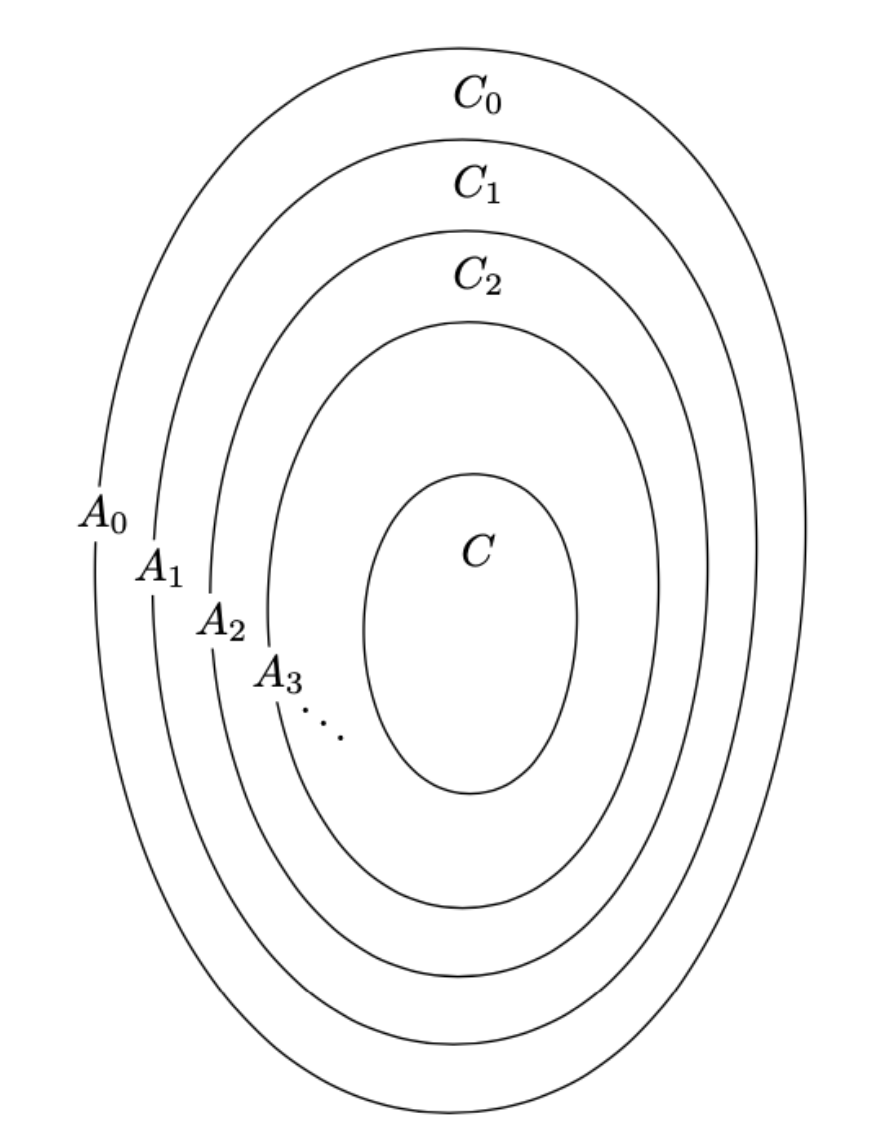
\includegraphics[width=0.5\linewidth]{Cantor.png}
\end{center}
\indent\textbf{Доказательство второй формулировки.} Пусть дана функция $g: X \rightarrow Y$, и $C \subseteq D \subseteq X$. Тогда $f[C] \subseteq f[D]$ (по определению образа)\\[2mm]
\indent По условию теоремы есть биекция $f: A_{0} \rightarrow A_{2}$. При такой биекции множество $A_{1}$ переходит в множество $A_{3} \subseteq A_{2}$ (то есть $A_{3}=f\left[A_{1}\right]$). Аналогичным образом $A_{2}$ переходит в множество $A_{4} \subseteq A_{3}$ (так как $A_{2} \subseteq A_{1}$,$\left.A_{4}=f\left[A_{2}\right], A_{3}=f\left[A_{1}\right]\right)$. Продолжая эту конструкцию, мы получаем убывающую последовательность множеств\\[2mm]
$$
A_{0} \supseteq A_{1} \supseteq A_{2} \supseteq A_{3} \supseteq A_{4} \supseteq \ldots
$$
\indent При этом $f\left[A_{i}\right]=A_{i+2}$. Самое большое множество $A_{0}$ разбито на непересекающиеся слои $C_{i}=A_{i} \backslash A_{i+1}$ и сердцевину $C=\bigcup_{i} A_{i}$\\[2mm]
\indent Слои $C_{0}, C_{2}, C_{4}, \ldots$ равномощны. Функция $f$ осуществляет биекцию между $A_{2 n}$ и $A_{2 n+2}$, и та же функция $f$ осуществляет биекцию между $A_{2 n+1}$ и $A_{2 n+3}$. При этом $A_{2 n+1} \subseteq A_{2 n}$ и $A_{2 n+3} \subseteq A_{2 n+2}$. Значит, функция $f$ осуществляет биекцию между $C_{2 n}=A_{2 n} \backslash A_{2 n+1}$ и $C_{2 n+2}=A_{2 n+2} \backslash A_{2 n+3}$:
$$
C_{0} \stackrel{f}{\longrightarrow} C_{2} \stackrel{f}{\longrightarrow} C_{4} \stackrel{f}{\longrightarrow} \ldots
$$
\indent То же самое можно сказать про слои с нечётными номерами:
$$
C_{1} \stackrel{f}{\longrightarrow} C_{3} \stackrel{f}{\longrightarrow} C_{5} \stackrel{f}{\longrightarrow} \ldots
$$
\indent Теперь можно построить биекцию $g: A_{0} \rightarrow A_{1}$. Пусть $x \in A_{0}$. Тогда $g(x)$ определяется так: если $x \in C_{2 k}$ при некотором $k$, то $g(x)=f(x)$, в противном случае (то есть если $x \in C_{2 k+1}$ при некотором $k$ или $x \in C$ ), то $g(x)=x$. \qed
\subsection{Примеры применения теоремы Кантора–Бернштейна: континуальность множества тотальных функций $\mathbb{N}\rightarrow\mathbb{N}$; равномощность квадрата и круга}
\textbf{Пример применения-1.} Континуальность множества тотальных функций $\mathbb{N}\rightarrow\mathbb{N}$\\[2mm]
\indent \textit{Док-во по второй формулировке.} Заметим, что $\{0,1\}^{\mathbb{N}}\subseteq\mathbb{N}^{\mathbb{N}}\subseteq\mathbb{R}^{\mathbb{N}}$. Действительно, любая функция $\mathbb{N}\rightarrow \{0,1\}$ является функцией $\mathbb{N}\rightarrow\mathbb{N}$, а любая функция $\mathbb{N}\rightarrow\mathbb{N}$ является функцией $\mathbb{N}\rightarrow\mathbb{R}$. По теореме \ref{sec:2.36} множество $\mathbb{R}^{\mathbb{N}}$ континуально, то есть равномощно $\{0,1\}^{\mathbb{N}}$. По теореме Кантора–Бернштейна $\mathbb{N}^{\mathbb{N}}$ равномощно $\{0, 1\}^{\mathbb{N}}$\\[2mm]
\textbf{Пример применения-2.} Квадрат (с внутренностью) равномощен кругу\\[2mm]
\indent Из круга можно вырезать маленький квадрат и устроить гомотетию\footnote{Гомотетия - преобразование плоскости, переводящее точку $M$ в $M_1$, т.ч. $\overrightarrow{OM_1}=k\overrightarrow{OM}$. $O$-центр, $k$-коэффициент, отличный от 0} с исходным квадратом. Аналогично, из квадрата можно вырезать маленький круг и устроить гомотетию с исходным кругом. Отсюда по теореме Кантора-Бернштейна (в первой формулировке) следует равномощность квадрата и круга
\subsection{Теорема Кантора и следствия из неё}
\textbf{Теорема.} Никакое множество $X$ не равномощно множеству $\mathcal{P}(X)$ своих подмножсеств\\[2mm]
\textit{Доказательство.} Пусть $f$ - тотальная функция из множества $X$ в $\mathcal{P}(X)$. Докажем, что она не сюръекция (значит, и не биекция). Для этого построим множество $Y \subseteq X$, отличающееся от $f(x)$ для всех $x \in X$. Чтобы задать $Y$, нужно пересказать диагональное рассуждение, переходя от бесконечных двоичных последовательностей к подмножествам $\mathbb{N}$. Мы его проводили, когда доказывали несчётность множества $\{0,1\}^{\mathbb{N}}$ (теорема \ref{sec:2.33})\\[2mm]
Рассмотрим множество
$$
Y=\{x \in X: x \notin f(x)\} .
$$
По построению множества $Y, x \in Y \Leftrightarrow x \notin f(x)$\\[2mm]
\indent Докажем, что $Y$ не лежит в образе $f[X]$, то есть отличается от любого $f(x)$, $x \in X$. Пусть это не так, тогда $Y=f(z)$ для некоторого $z \in X$. Тогда
$$
z \in Y \Leftrightarrow z \notin f(z) \Leftrightarrow z \notin Y
$$
(первое - по построению множества $Y$, второе - по предположению $f(z)=Y$ ). Пришли к противоречию. Следовательно, $Y$ ничему не соответствует. \qed\\[2mm]
\textbf{Следствия из теоремы.}\\[2mm]
\indent 1. Для любого множества $X$ имеем $|X|<|\mathcal{P}(X)|$\\[2mm]
\indent 2. Для любого натурального числа $n$ выполнено $n<2^{n}$\\[2mm]
\indent 3. Множества всех множеств не существует\\[2mm]
\textit{Доказательства следствий.}\\[2mm]
\indent 1. По теореме Кантора, не существует биекции между $X$ и $\mathcal{P}(X)$. С другой стороны, существует инъекция $f: X \rightarrow \mathcal{P}(X): f(x)=\{x\}$. Поэтому по определению $|X|<|\mathcal{P}(X)|$. \qed\\[2mm]
\indent 2. Рассмотрим конечное множество $X$ из $n$ элементов. По предыдущему следствию, $|X|<|\mathcal{P}(X)|$. В множестве $\mathcal{P}(X)$ имеется $2^{n}$ элементов. Отсюда получаем, что $n<2^{n}$. \qed\\[2mm]
\indent 3. От противного: предположим, что совокупность всех множеств $U$ является множеством. Заметим, что все подмножества множества $U$ (и вообще все подмножества любых множеств!) являются его элементами. Поэтому множество $\mathcal{P}(U)$ всех подмножеств $U$ является подмножеством $U$. Значит, есть инъекция $\mathcal{P}(U) \rightarrow U$. В обратную сторону инъекция есть всегда: для любого множества $X$ отображение $x \mapsto\{x\}$ является инъекцией $X$ в $\mathcal{P}(X)$. По теореме Кантора-Бернштейна $U$ равномощно $\mathcal{P}(U)$, что противоречит теореме Кантора. \qed
\subsection{Критерий транзитивности отношения. Отношение, являющееся одновременно рефлексивным и антирефлексивным. Отношение, являющееся одновременно симметричным и антисимметричным. Транзитивность пустого и одноэлементного отношения}
\label{sec:2.41}\textbf{Утверждение.} Отношение $R$ на множестве $A$ транзитивно тогда и только тогда, когда $R\circ R\subseteq R$\\[2mm]
\textbf{Доказательство.} Пусть отношение $R$ транзитивно. Рассмотрим какую-нибудь пару $(a, b)\subseteq R\circ R$. Это означает, что для некоторого $y\subseteq A (a, y), (y, b) \in R$. По транзитивности $R$ получаем, что $(a, b)\in R$. Значит, выполняется включение $R\circ R\subseteq R$\\[2mm] 
\indent Обратно, пусть $R\circ R\subseteq R$. Возьмём две пары $(x, y)$ и $(y, z)$ из отношения $R$. По определению композиции $(x, z)\in R\circ R$. Поскольку квадрат отношения лежит в нём самом, получаем, что $(x, z)\in R$. То есть доказали транзитивность отношения. \qed\\[2mm]
\indent\textbf{Пример-1.} Нужно, чтобы $\forall x\in A$ было выполнено $(x, x)\in R$ и $(x, x)\notin R$. Это невозможно, если в множестве $A$ содержится хотя бы один элемент. Если же множество $A$ пусто, то единственное бинарное отношение на множестве $A$ — это пустое отношение. Оно является одновременно и рефлексивным, и антирефлексивным\\[2mm]
\indent\textbf{Пример-2.} Пусть какое-то $(x, y)\in R$. В силу симметричности $(y, x)\in R$, а в силу антисимметричности получаем, что $x=y$. Таким образом, если $R$ одновременно симметрично и антисимметрично, то в него могут попасть только пары вида $(x, x)$, то есть $R\subseteq id_A$. Обратно: ясно, что любое бинарное отношение $R$, для которого выполнено $R\subseteq id_A$, является одновременно симметричным и антисимметричным\\[2mm]
\indent\textbf{Пример-3.} Пустое бинарное отношение $\varnothing$ на любом множестве $A$ является транзитивным, потому что в импликации $(x,y)\in\varnothing\wedge(y,z)\in\varnothing\rightarrow(x,z)\in\varnothing$ левая часть всегда ложна, а импликация всегда истинна. Можно также сказать, что $\varnothing\circ\varnothing = \varnothing$, то есть выполнен критерий транзитивности. Любое отношение, содержащее ровно одну пару, также является транзитивным. Пусть $R = \{(a, b)\}$. Тогда, если $a\ne b$, то $R\circ R = \varnothing$, а если $a = b$, то $R\circ R = \{(a, a)\}$. То есть снова выполнен критерий транзитивности $R\circ R\subseteq R$
\subsection{Выражение композиции отношений через матрицы. Критерий транзитивности отношения в терминах матриц}
Пусть $M_{R}$ и $M_{S}$ - матрицы отношений $R$ и $S$ ($R$ - бинарное отношение на множествах $A$ и $B, S-$ бинарное отношение на множествах $B$ и $C$, элементы множества $B$ в обеих матрицах пронумерованы одинаково)\\[2mm]
\indent Тогда матрица отношения $S \circ R$ получается так: берём матрицу $M_{R} \cdot M_{S}$, после чего меняем все числа, превосходящие 1, на 1. Пусть $\left(a_{i}, c_{k}\right) \in S \circ R$. Ээто означает, что $\exists$ $b_{j}$, что $\left(a_{i}, b_{j}\right) \in R,\left(b_{j}, c_{k}\right) \in S$. Значит, при вычислении элемента $(i, k)$ матрицы $M_{R} \cdot M_{S}$ в сумме $\sum_{l} M_{R}(i, l) M_{S}(l, k)$ возникло ненулевое число. А значит, элемент $(i, k)$ матрицы $M_{R} \cdot M_{S}$ будет положительным. Аналогично рассуждаем, если $\left(a_{i}, c_{k}\right) \notin S \circ R$\\[2mm]
\indent Пусть $M$ — матрица бинарного отношения $R$. Пусть матрица $N$ получается из матрицы $M\cdot M$ заменой всех элементов, больших 1, на 1. Тогда отношение $R$ транзитивно тогда и только тогда, когда в матрице $N$ каждый элемент не превосходит элемента матрицы $M$, стоящего на том же месте (иными словами, не бывает такого, что в матрице $N$ стоит 1 на том месте, где в матрице $M$ стоит 0). Это наблюдение следует из утверждения \ref{sec:2.41} и того, как считается матрица композиции\\[2mm]
\textbf{Пример.} Пусть матрица отношения $R$ равна $\begin{pmatrix}
    1&1\\
    1&0
\end{pmatrix}$. Тогда матрица отношения $R\circ R:\begin{pmatrix}
    1&1\\
    1&0
\end{pmatrix}\begin{pmatrix}
    1&1\\
    1&0
\end{pmatrix}=\begin{pmatrix}
    2&1\\
    1&1
\end{pmatrix}\rightarrow\begin{pmatrix}
    1&1\\
    1&1
\end{pmatrix}$. На месте (2,2) в этой матрице стоит 1, а в исходной — 0\\[2mm]
Следовательно, $R$ не транзитивно
\subsection{Свойства транзитивного замыкания. Транзитивность пересечения любого непустого семейства транзитивных отношений. Существование и единственность транзитивного замыкания}
Свойства транзитивного замыкания приведены здесь - \ref{sec:1.62}\\[2mm]
\indent\textbf{Доказательства}\\[2mm]
\indent 1. Пусть $R$ - транзитивно. Проверим, что $R$ - его транзитивное замыкание. Действительно, $R$ транзитивно, $R \subseteq R$, и для любого транзитивного $T$, если $R \subseteq T$, то $R \subseteq T$. Значит, по определению, $R^{*}=R$\\[2mm]
\indent 2. По определению $R^{*}$ транзитивно. Осталось применить п. 1\\[2mm]
\indent\textbf{Лемма о транзитивности пересечения непустого...} Пусть $R_{i}, i \in I-$ произвольный непустой набор транзитивных отношений на множестве $A$. Тогда их пересечение $\bigcap_{i \in I} R_{i}$ также транзитивно (это также отношение на множестве $A$)\\[2mm]
\indent\textbf{Доказательство.} Возьмём любые $(x, y),(y, z) \in \bigcap_{i \in I} R_{i}$. Раз они лежат в пересечении, то они лежат в каждом $R_{i}$. Так как каждое $R_{i}$ транзитивно, имеем $(x, z) \in R_{i}$ для всех $i$. Отсюда $(x, z) \in \bigcap_{i \in I} R_{i}$. \qed\\[2mm]
\indent\textbf{Теорема о существовании и единственности транзитивного замыкания.} Для любого бинарного отношения $R$ на множестве А существует его транзитивное замыкание $R^{*}$\\[2mm]
\indent\textbf{Доказательство.} Рассмотрим все транзитивные отношения $R_{i}$ на множестве $A$, содержащие отношение $R$ (обозначим $i \in I$ ). Этот набор непуст: ему точно принадлежит полное бинарное отношение. Значит, можно рассмотреть его пересечение $\bigcap_{i \in I} R_{i}$\\[2mm]
\indent По предыдущей лемме это отношение также транзитивно. Далее, поскольку $R \subseteq R_{i}$ для каждого $i$, то $R \subseteq \bigcap_{i \in I} R_{i}$. Наконец, если $T$ - какое-то транзитивное отношение на множестве $A$, то оно присутствует в этом наборе $R_{i}, i \in I$. А это означает, что $\bigcap_{i \in I} R_{i} \subseteq T$. \qed\\[2mm]
\indent Единственность транзитивного замыкания легко следует из определения. Действительно, если бы $R_{1}^{*}$ и $R_{2}^{*}$ были бы транзитивными замыканиями отношения $R$, то тогда имеем $R_{1}^{*} \subseteq R_{2}^{*}$ и $R_{2}^{*} \subseteq R_{1}^{*}$, откуда следует, что $R_{1}^{*}=R_{2}^{*}$
\subsection{Построение транзитивного замыкания по заданному отношению}
Пусть $R$ - бинарное отношение на множестве А. Тогда
$$
R^{*}=R \cup R^{2} \cup R^{3} \cup \ldots R^{n} \cup \ldots
$$
\indent\textbf{Доказательство.} Пусть $T$ - бинарное отношение $R \cup R^{2} \cup R^{3} \cup \ldots R^{n} \cup \ldots$. Докажем, что $R^{*}=T$\\[2mm]
\indentДокажем, что $T$ транзитивно. Возьмём произвольные $(x, y),(y, z) \in T$. Тогда существуют $k, s \in \mathbb{N}$, что $(x, y) \in R^{k},(y, z) \in R^{s}$. Отсюда $(x, z) \in R^{k+s}$, а, значит, $(x, z) \in T$\\[2mm]
\indentПоскольку $T$ транзитивно, отсюда немедленно получаем, что $R^{*} \subseteq T$\\[2mm]
\indentДокажем, что для любого $n \in \mathbb{N} \setminus\{0\}$ выполнено $R^{n} \subseteq R^{*}$ (следоватьно, $T \subseteq R^{*}$)\\
База очевидна: $R^{1}=R \subseteq R^{*}$ по определению транзитивного замыкания. Шаг: пусть $R^{n} \subseteq R^{*}$. Возьмём произвольное $(x, z) \in R^{n+1}$. Поскольку $R^{n+1}=R \circ R^{n}$, по определению композиции отношений существует $y$, для которого $(x, y) \in R^{n}$ и $(y, z) \in R$. По предположению индукции $(x, y) \in R^{*}$ и $(y, z) \in R^{*}$. Так как $R^{*}$ транзитивно, получаем, что $(x, z) \in R^{*}$. Таким образом, доказано, что $R^{n+1} \subseteq R^{*}$\\[2mm]
\indent Поскольку доказаны оба включения $R^{*} \subseteq T$ и $T \subseteq R^{*}$, заключаем, что $T=R^{*}$. \qed\\[2mm]
\textbf{Примечание.} Если множество $A$ конечно, то отношения в бесконечной цепочке $$R \cup R^{2} \cup R^{3} \cup \ldots R^{n} \cup \ldots$$ с какого-то места начнут повторяться, потому что существует только конечное множество бинарных отношений на конечном множестве $A$. Так что для конечных множеств это будет по существу конечное объединение
\subsection{Теорема о сумме степеней вершин. Лемма о рукопожатиях. Число рёбер в полном графе на n вершинах, число рёбер в булевом кубе}
Теорема и лемма приведены тут - \ref{sec:1.65}\\[2mm]
\textbf{Доказательство теоремы}\\[2mm]
\indentПрименим метод двойного подсчёта. Под таким громким названием скрывается очень простой факт: если посчитать сумму элементов матрицы по строкам, то получится такое же число, как и при суммировании элементов матрицы по столбцам\\[2mm]
\indentДавайте посчитаем количество 1 в матрице инцидентности графа. В строке $i$ количество 1 равно количеству инцидентных вершине $i$ рёбер, то есть степени этой вершины. Значит, сумма 1 по строкам равна сумме степеней вершин\\[2mm]
\indentВ каждом столбце матрицы инцидентности ровно две 1 , так как у ребра ровно два конца. Значит, сумма 1 по столбцам равна удвоенному количеству рёбер\\[2mm]
\indentОбе суммы равны общему количеству 1 в матрице инцидентности, а значит, равны между собой. \qed\\[7mm]
\textbf{Доказательство леммы}\\[2mm]
\indent Эта лемма следует из предыдущей теоремы. Сумма степеней всех вершин - это всегда чётное число, поэтому нечётных слагаемых в этой сумме должно быть чётное количество\\[2mm]
\textbf{Число ребер в полном графе.} В полном графе $K_{n}$ имеется $n$ вершин, и каждая пара вершин соединена ребром\\[2mm]
\indent Степень каждой вершины равна $(n-1)$ (вершина связана ребром со всеми остальными). Поэтому сумма степеней вершин равна $n(n-1)$. А количество рёбер в два раза меньше: $\frac{n(n-1)}{2}$\\[2mm]
\textbf{Число ребер в булевом кубе.} Вершины булева куба $Q_{n}$ (булев куб размерности $n$)двоичные слова длины $n$. Два слова $u$ и $v$ соседние в булевом кубе, если и только если одно можно получить из другого инвертированием ровно одной позиции. (Инвертирование означает изменение значения: с 0 на 1 или с 1 на 0)\\[2mm]
\indent Скажем, 0100 и 0101 соседние в $Q_{4}$, а 0100 и 0011 - нет\\[2mm]
\indentКоличество вершин в булевом кубе $Q_{n}$ равно $2^{n}$, это количество двоичных слов длины $n$\\[2mm]
\indent Степень каждой вершины равна $n$ : есть ровно $n$ позиций, инвертирование каждой даёт соседа и других соседей нет. Поэтому количество рёбер в булевом кубе $Q_{n}$ равно $n 2^{n} / 2=n 2^{n-1}$
\subsection{Связность графа перестановок, в котором проведены рёбра между перестановками, получающимися друг из друга переворотом начального отрезка}
Множество вершин графа $F_{n}$ - это множество $S_{n}$ всех перестановок на множестве $\{1,2, \ldots, n\}$. Удобнее представлять перестановки как размещения из $n$ по $n$. Две перестановки связаны ребром в графе $F_{n}$, если одна получается из другой переписыванием некоторого начального отрезка перестановки в обратном порядке (назовём такое преобразование переворотом). Вот пример переворота:
$$
(4,3,2,6,1,5) \rightarrow(6,2,3,4,1,5)
$$
\indentДокажем, что переворотами можно упорядочить любую последовательность\\[2mm]
\indentДоказательство индукцией по $n$. База $n=2$ очевидна: есть всего две перестановки и одна получается из другой переворотом всей последовательности\\[2mm]
\indentШаг индукции. Предполагаем, что любую перестановку чисел из $\{1,2, \ldots, n\}$ возможно упорядочить переворотами. Рассмотрим перестановку чисел из $\{1,2, \ldots, n+1\}$. Выделим в ней начальный отрезок, заканчивающийся $n+1:\left(x_{1}, \ldots, x_{i}, n+1, x_{i+1}, \ldots, x_{n}\right)$. Выполним переворот этого отрезка, а затем переворот всей последовательности, получаем
$$
\begin{aligned}
\left(x_{1}, \ldots, x_{i}, n+1, x_{i+1}, \ldots, x_{n}\right) \rightarrow\left(n+1, x_{i}, \ldots, x_{1}, x_{i+1}, \ldots, x_{n}\right) \rightarrow & \\
& \rightarrow\left(x_{n}, \ldots, x_{i+1}, x_{1}, \ldots, x_{i}, n+1\right)
\end{aligned}
$$\\[2mm]
\indentВ полученной перестановке $n+1$ уже стоит на своём месте. Пользуясь индуктивным предположением, упорядочим теперь начальный отрезок длины $n$\\[2mm]
\indentОтсюда легко получить связность графа $F_{n}$. Из любых двух перестановок $\pi, \sigma$ существуют пути в $(1,2, \ldots, n)$. Путь из $\pi, \sigma$ получается соединением пути из $\pi$ в $(1,2, \ldots, n)$ и переворотом пути из $\sigma$ в $(1,2, \ldots, n)$.
\subsection{Свойства отношения достижимости в графе. Построение отношения эквивалентности по разбиению множества}
Свойства отношения приведены тут - \ref{sec:1.67}\\[2mm]
\textbf{Доказательство свойств}\\[2mm]
\indentТак как $v$ - путь (длины 0 ), вершина $v$ связанная с самой собой\\[2mm]
\indentЕсли $v_{1} u_{1} \ldots u_{s} v_{2}$-путь в графе, то $v_{2} u_{s} \ldots u_{1} v_{1}$-также путь (записываем те же вершины, но в обратном порядке). Поэтому достижимость $v_{2}$ из $v_{1}$ равносильна достижимости $v_{1}$ из $v_{2}$\\[2mm]
\indent Если в графе есть пути $v_{1} u_{1} \ldots u_{s} v_{2}$ и $v_{2} w_{1} \ldots w_{t} v_{3}$ (то есть $\left(v_{1}, v_{2}\right) \in R$ и $\left.\left(v_{2}, v_{3}\right) \in R\right)$, то в этом графе есть также и путь $v_{1} u_{1} \ldots u_{s} v_{2} w_{1} \ldots w_{t} v_{3}$, то есть $\left(v_{1}, v_{3}\right) \in R$ (вершина $v_{3}$ достижима из $\left.v_{1}\right)$. \qed\\[2mm]
Пример описан здесь - \ref{sec:1.68}
\subsection{Теорема о том, что отношение эквивалентности делит множество на классы эквивалентности}
Теорема сформулирована тут - \ref{sec:1.69}\\[2mm]
\textbf{Доказательство.} Для каждого $x \in A$ рассмотрим множество $C(x)=\{y: x R y\}$ тех $y$, для которых верно $x R y$. Это и есть обещанные классы эквивалентности. Чтобы это доказать, нужно проверить три условия:\\[2mm]
\indent 1. Объединение всех множеств вида $C(x)$ совпадает с множеством $A$\\[2mm]
\indent 2. Два множества $C(x)$ и $C(y)$ либо не пересекаются, либо совпадают\\[2mm]
\indent 3. $C(x)=C(y)$ в том и только том случае, когда $x R y$ (то есть $R$ совпадает с отношением «принадлежать одному классу», как в примере \ref{sec:1.68})\\[2mm]
\indent 1. В силу рефлексивности множество $C(x)$ содержит $x$ в качестве своего элемента: $x \in C(x)$, поскольку $x R x$. Отсюда следует, что объединение всех этих множеств совпадает с $A$\\[2mm]
\indent2. Пусть $z \in C(x) \cap C(y)$, то есть верно $x R z$ и $y R z$. Симметричность даёт $z R y$. Теперь применим транзитивность к $x R z$ и $z R y$, заключаем, что $x R y$ и по симметричности $y R x$\\[2mm]
\indentПусть $t \in C(y)$, то есть $y R t$. Применим транзитивность к $x R y$ и $y R t$, заключаем, что $x R t$, то есть $t \in C(x)$. Значит, $C(y) \subseteq C(x)$. Аналогично доказывается, что $C(x) \subseteq C(y)$, так что $C(x)=C(y)$\\[2mm]
\indent3. Если для каких-то $x, y$ верно $x R y$, то $x$ и $y$ оба лежат в одном классе, а именно, в $C(x)$. Обратно, если $x$ и $y$ лежат в каком-то $C(z)$, то по определению имеем $z R x$ и $z R y$. Симметричность даёт $x R z$, после чего транзитивность даёт $x R y$. \qed

\end{document}



: $\wedge, \vee, \rightarrow, \equiv, \neg$